\documentclass[10pt]{report}

\usepackage{stan-talks}

\begin{document}
\sf



% TITLE SLIDE
%
\vspace*{-12pt}
\noindent
\spc{\LARGE\bfseries \color{MidnightBlue}{Stan:}}
\\[3pt]
\spc{\large\bfseries \color{MidnightBlue}{Probabilistic Modeling
    \& Bayesian Inference}}
\\[12pt]
\noindent
\spc{\bfseries Development Team}
  \\[2pt]
  \spc{\footnotesize Andrew Gelman, \ \myemph{Bob Carpenter}, \ Daniel
    Lee, \ Ben Goodrich, }
  \\
  \spc{\footnotesize Michael Betancourt, \ Marcus Brubaker, \ Jiqiang
    Guo, \ Allen Riddell,}
  \\
  \spc{\footnotesize Marco Inacio, \ Jeffrey Arnold, \ \myemph{Mitzi Morris}, \
    Rob Trangucci,}
  \\
  \spc{\footnotesize Rob Goedman, \ Brian Lau, \, Jonah Sol Gabry, \
    Robert L.\ Grant, \ }
  \\
  \spc{\footnotesize Krzysztof Sakrejda, \ Aki Vehtari, \ Rayleigh
    Lei, \ Sebastian Weber, }
  \\
  \spc{\footnotesize Charles Margossian, \ Vincent Picaud, \ Imad
    Ali, \ \myemph{Sean Talts},}
  \\
  \spc{\footnotesize Ben Bales, \ Ari Hartikainen, \ Matthijs
    V\`ak\`ar, \ Andrew Johnson,}
  \\
  \spc{\footnotesize Dan Simpson}
\\[-20pt] \noindent
  \spc{\small Stan 2.17 \ \footnotesize (November 2017)
    \hfill \url{http://mc-stan.org}} \hfill

\includegraphics[width=0.45in]{img/new-logo.png}


\mypart{Stan}{Who, What, and Why?}

\sld{Who is Stan?}
%
\begin{itemize}
\item Stan is named in honor of \myemph{Stanislaw Ulam} (1909--1984)
\item Co-inventor of the \myemph{Monte Carlo method}
\item[]
\vspace*{4pt}
  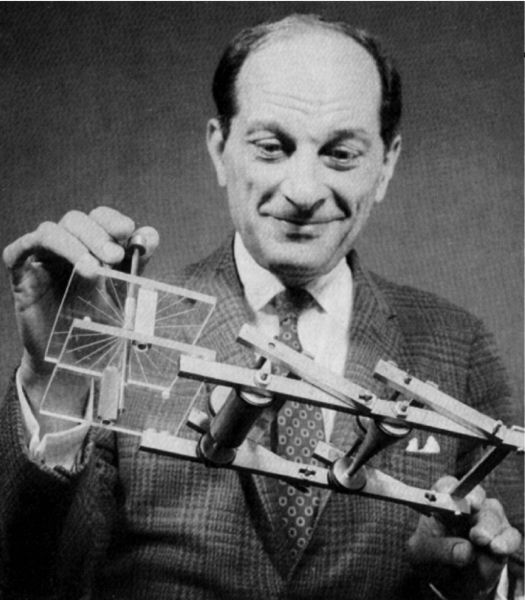
\includegraphics[width=0.25\textwidth]{img/ulam-fermiac.jpg}
\\[2pt] \footnotesize Ulam holding the Fermiac, Enrico Fermi's physical Monte Carlo simulator
  for random neutron diffusion; \hfill
\\[4pt]
{\tiny \mbox{ } \hfill image from G.~C.~Geisler (2000) Los Alamos report LA-UR-2532}
\end{itemize}

\sld{What is Stan?}
%
\begin{itemize}
\item Stan is an \myemph{imperative probabilistic programming language}
  \begin{subitemize}
  \item  cf., BUGS: declarative; \ Church: functional; \ Figaro: OO
  \end{subitemize}
\item Stan \myemph{program}: defines a probability model
  \begin{subitemize}
  \item declares data and (constrained) parameter variables
  \item defines log posterior (or penalized likelihood)
  \end{subitemize}
\item Stan \myemph{inference}: fits model to data \& makes predictions
  \begin{subitemize}
  \item MCMC for full Bayesian inference
  \item VB for approximate Bayesian inference
  \item MLE for penalized maximum likelihood estimation
  \end{subitemize}
\end{itemize}


\sld{Why Choose Stan?}
%
\begin{itemize}
\item \myemph{Expressive}
\begin{subitemize}
\item Stan is a full imperative programming language
\item continuously differentiable log densities
\end{subitemize}
\item \myemph{Robust}
\begin{subitemize}
\item usually works; signals when it doesn't
\end{subitemize}
\item \myemph{Efficient}
\begin{subitemize}
\item effective sample size / time (i.e., information)
\item multi-core and GPU code complete on branches
\end{subitemize}
\item Ongoing \myemph{open source} development
\item \myemph{Community} support!
\end{itemize}


\sld{What's Next for Stan?}
%
\begin{itemize}
\item Distributed likelihoods: \myemph{multi-CPU} (MPI)
\item Big matrix operations: \myemph{GPU} (OpenCL)
\item Sparse matrix operations
% \item Streaming data: \myemph{stochastic variational} inference
\item Distributed data: asynchronous \myemph{expectation propagation}
\item Approximations: parallel \myemph{max marginal mode}
\item \myemph{Coursera} specialization
\begin{subitemize}
\item Gelman: Bayesian data analysis, Multilevel regression
\item Carpenter: Monte Carlo methods, Stan
\item Fall 2018
\end{subitemize}
\end{itemize}



\mypart{}{Predator-Prey Dynamics}


\sld{Lynxes and Hares}
%
\begin{center}
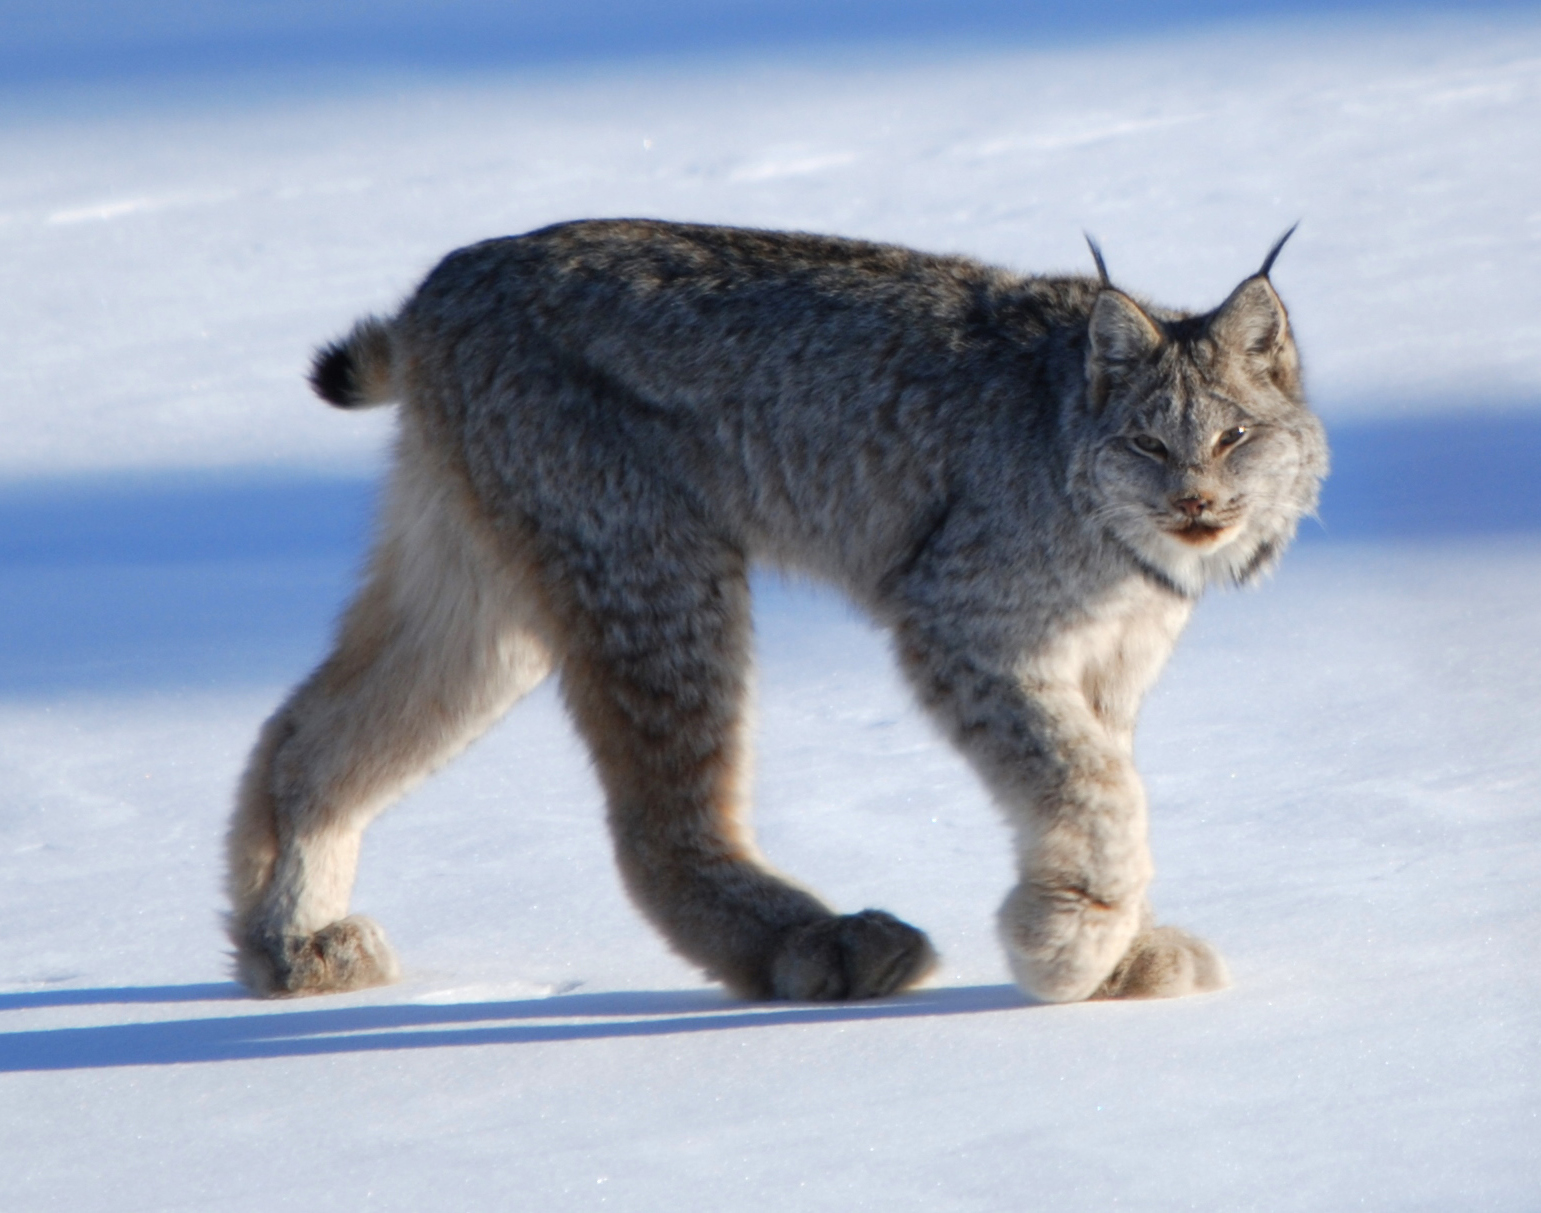
\includegraphics[height=1in]{img/lynx.jpg}
\hspace*{0.25in}
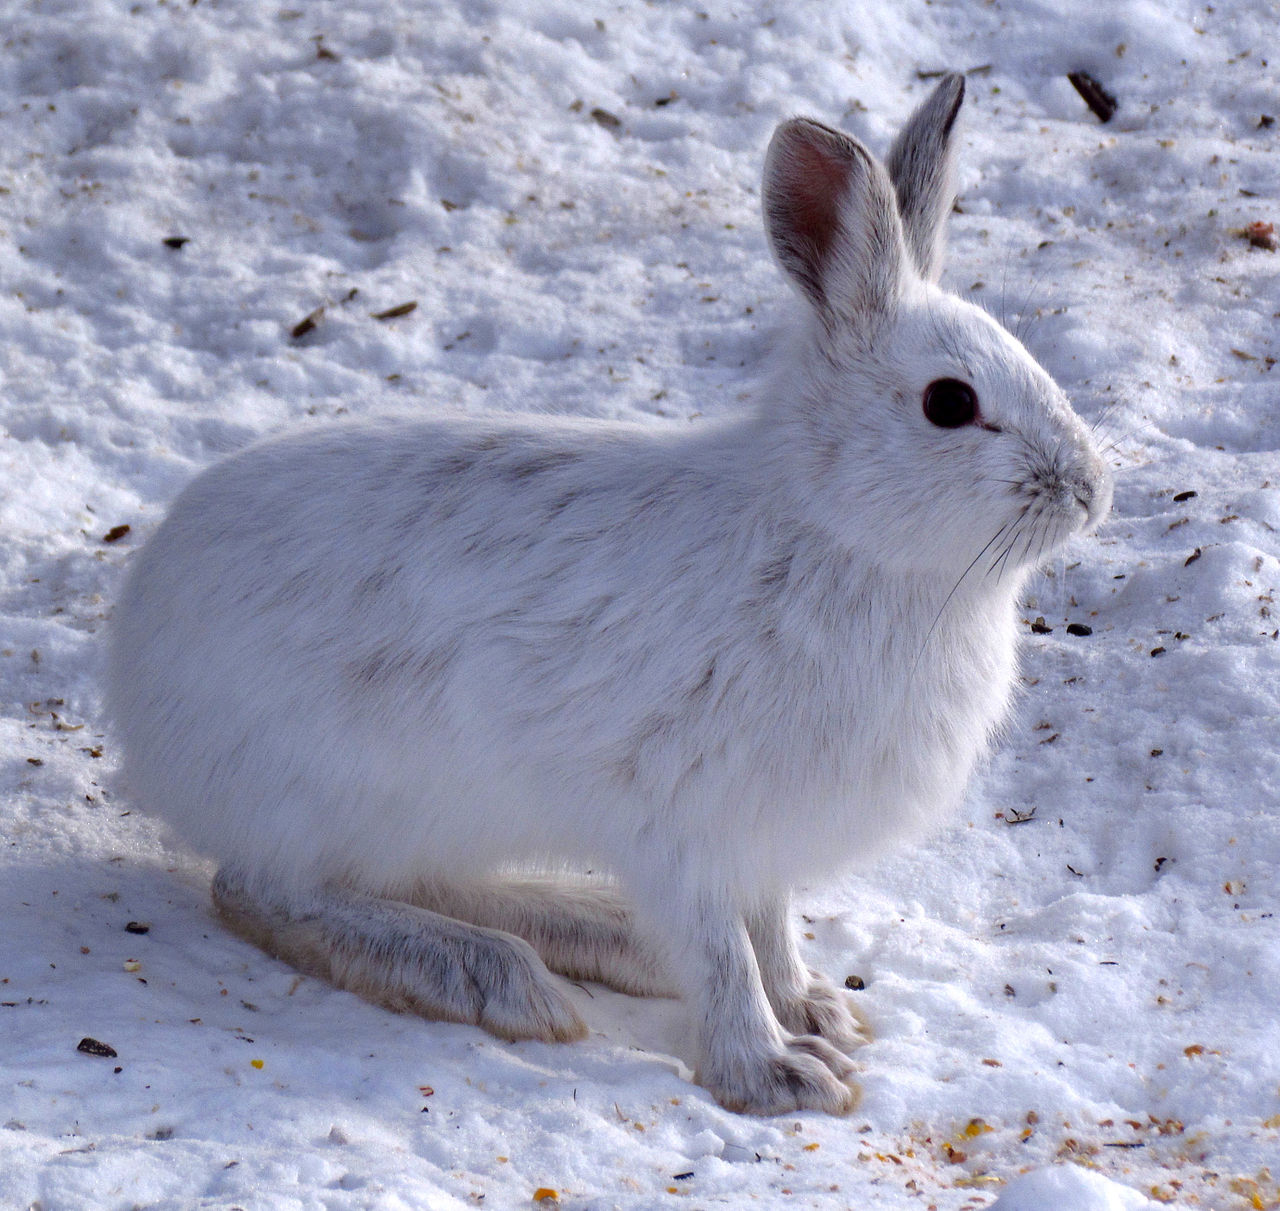
\includegraphics[height=1in]{img/hare.jpg}
\end{center}
\begin{itemize}
\item \myemph{Snowshoe hare} (prey): herbivorous cousin of rabbits
\item \myemph{Canadian lynx} (predator): feline eating primarily hares
\end{itemize}
\vfill
{\tiny
\mbox{ } \hfill
Lynx image copyright 2009, Keith Williams, CC-BY 2.0.
\\[-2pt]
\mbox{ } \hfill
Hare image copyright 2013 D. Gordon E. Robonson, CC-BY SA 2.0}


\sld{Hudson Bay Co. Pelts, 1900--20}
%
\\[-4pt] \spc
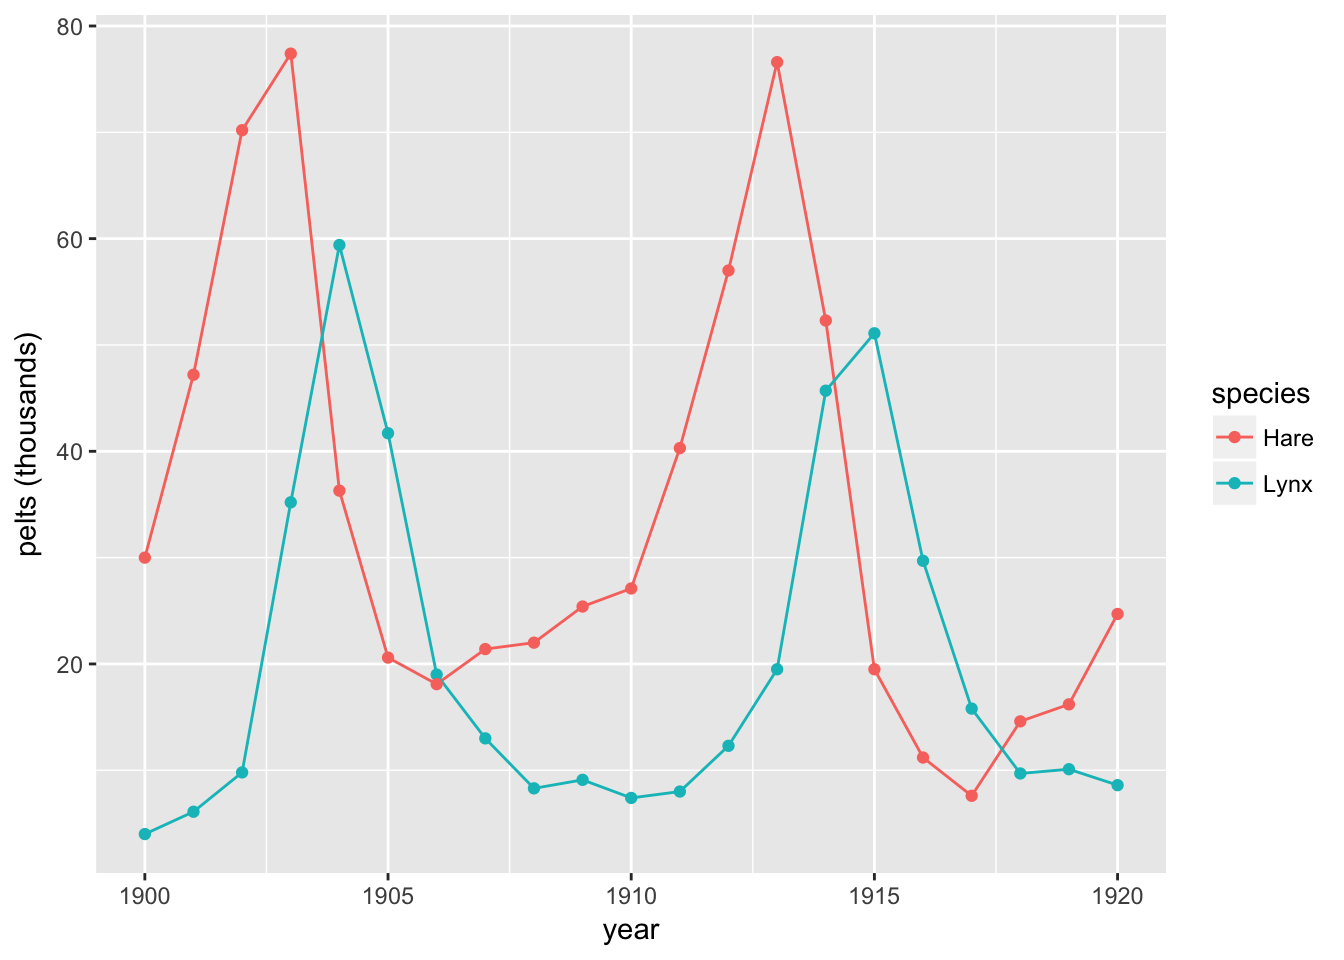
\includegraphics[width=0.85\textwidth]{img/hare-lynx-pelts-1.png}


\sld{Pelts, Phase Space}
%
\\[-4pt] \spc
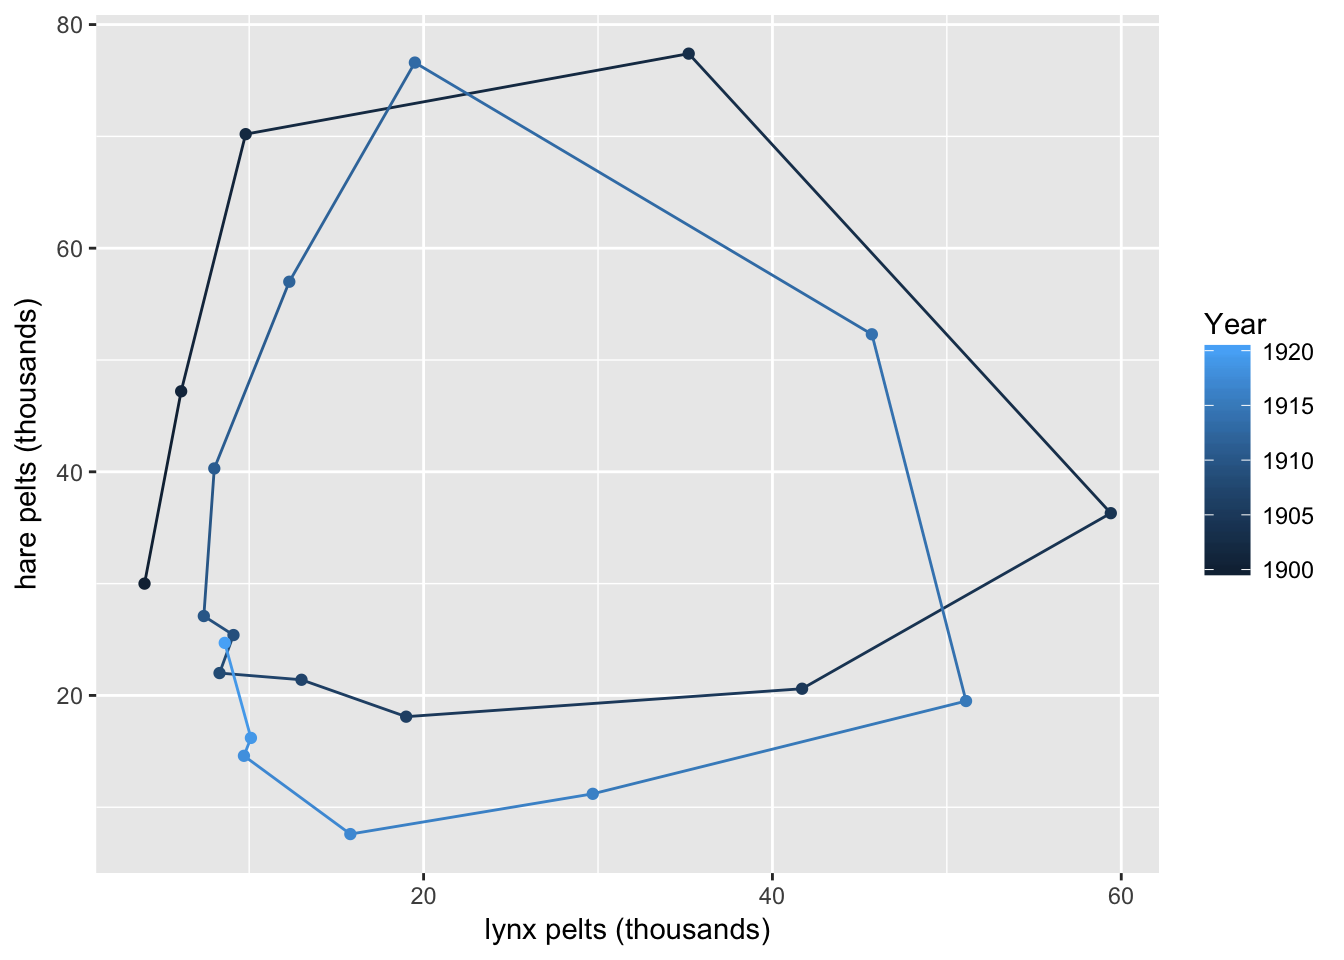
\includegraphics[width=0.85\textwidth]{img/hare-lynx-pelts-2.png}


\sld{Volterra's (1927) Model}
%

\begin{minipage}[t]{0.65\textwidth}
\vspace*{-1in}
\begin{subitemize}
\item population: $u(t)$ \myemph{prey}, \ $v(t)$ \myemph{predator}
%
\begin{eqnarray*}
\frac{\mathrm{d}}{\mathrm{d}t} u
& = &  (\alpha - \beta v) u
\\[6pt]
\frac{\mathrm{d}}{\mathrm{d}t} v
& = &  (-\gamma + \delta \, u) \, v
\end{eqnarray*}
%
\begin{subsubitemize}
\item $\alpha$: prey growth, intrinsic
\item $\beta$: prey shrinkage due to predation
\item $\gamma$: predator shrinkage, intrinsic
\item $\delta$: predator growth from predation
\end{subsubitemize}
\vspace*{-8pt}
\item \footnotesize dynamics lead to \myemph{oscillation} as observed
\end{subitemize}
\end{minipage}
%
\hfill
%
\begin{minipage}[t]{0.3\textwidth}
\mbox{ }
\vspace*{0.5in}
\mbox{ } \hfill
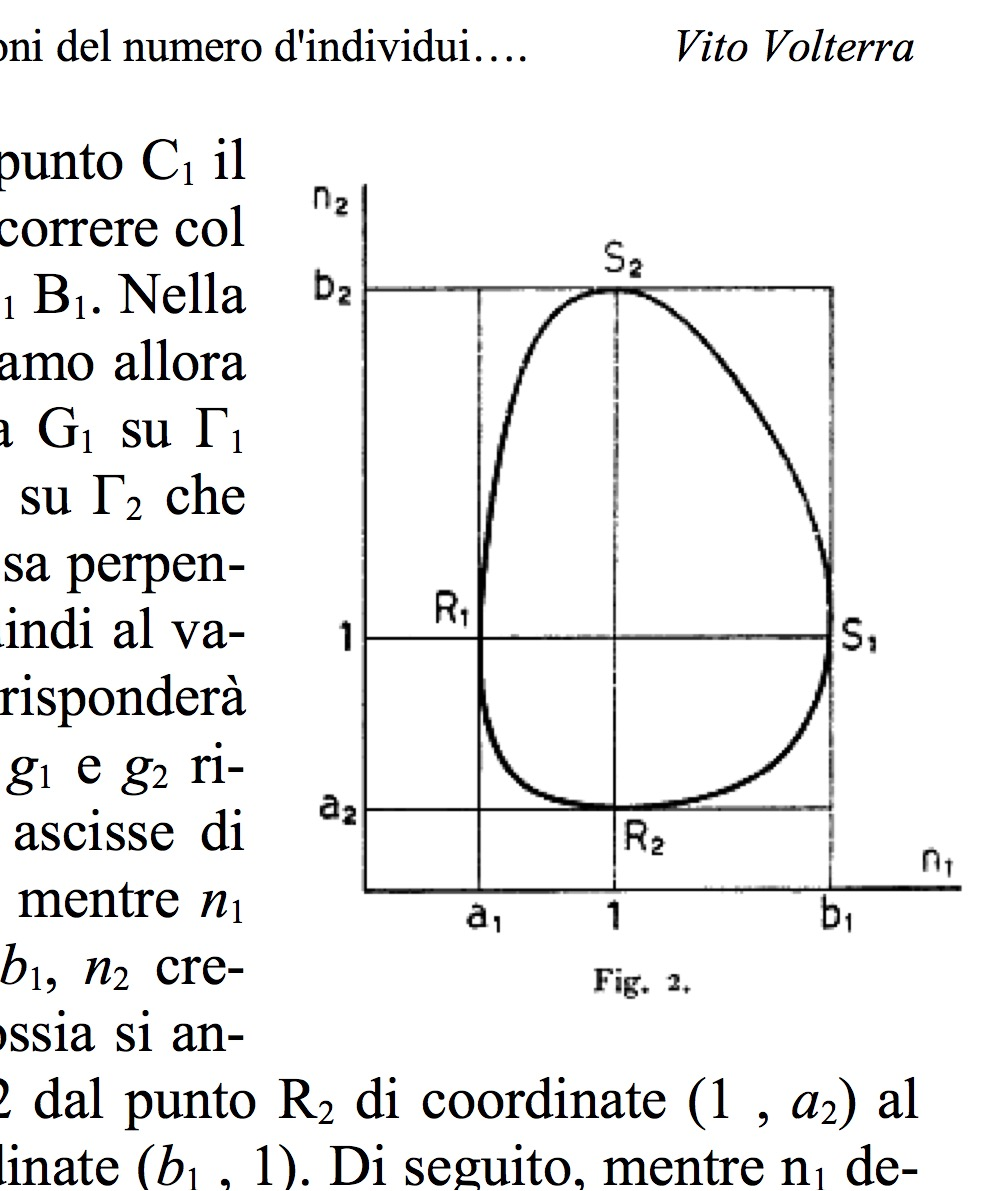
\includegraphics[width=0.8\textwidth]{img/volterra-orbit.jpg}
\\[-8pt]
\mbox{ }
\hfill
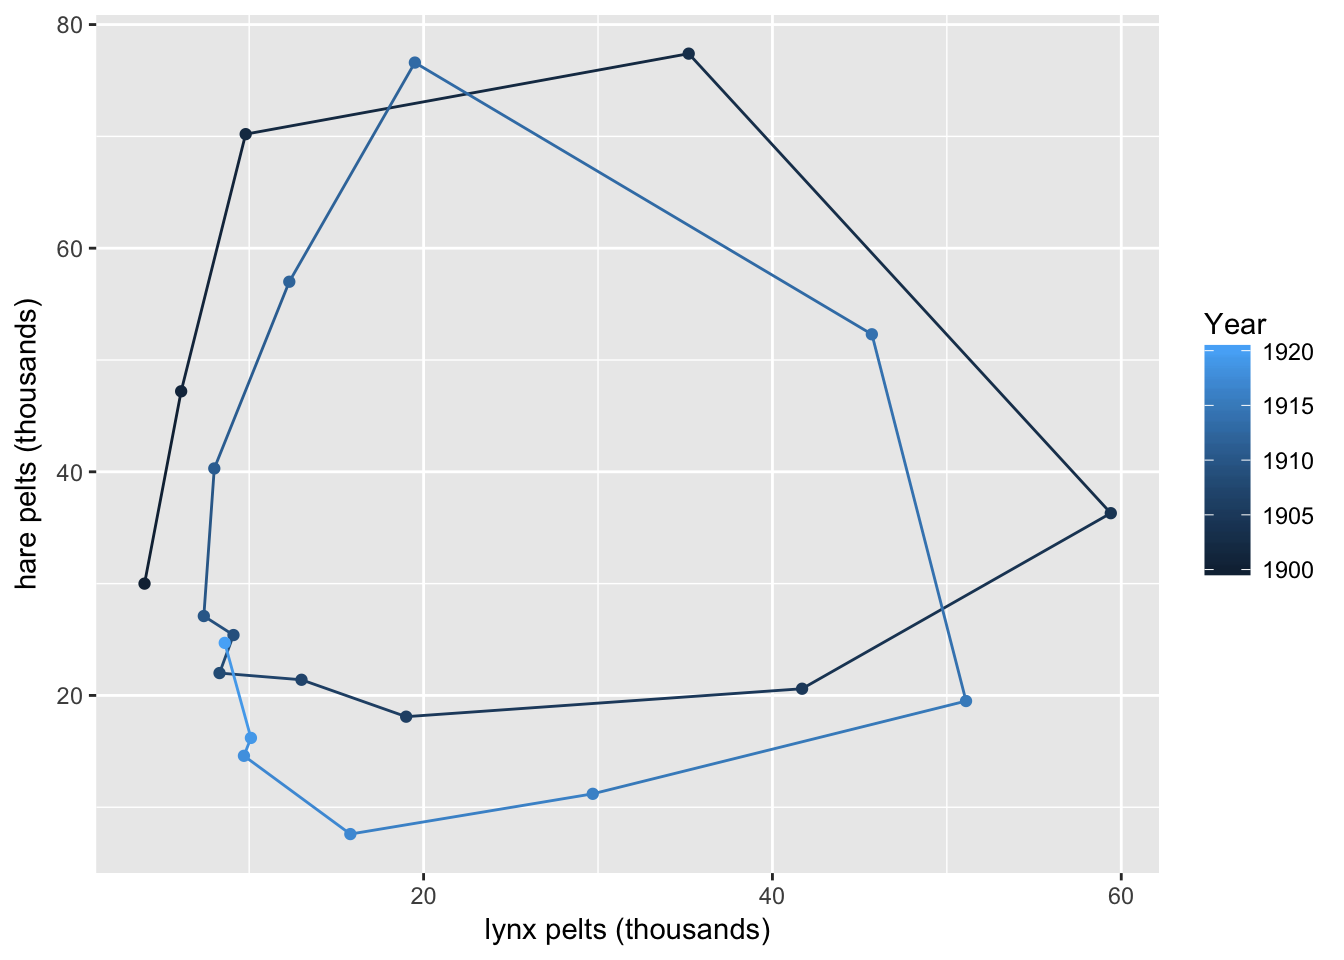
\includegraphics[width=0.8\textwidth]{img/hare-lynx-pelts-2.png}
\end{minipage}
\vfill
\hfill
{\tiny
Volterra, V., 1927. {\slshape Variazioni
e fluttuazioni del numero d'individui in specie animali
conviventi}. C.~Ferrari.
}



\sld{\Large Lotka-Volterra in Stan (dynamics)}
%
\vspace*{-2pt}
{\footnotesize
\begin{stancode}
  real[] dz_dt(data real t,       // time (unused)
               real[] z,          // system state
               real[] theta,      // parameters
               data real[] x_r,   // real data (unused)
               data int[] x_i) {  // integer data (unused)
    real u = z[1];                // extract state
    real v = z[2];

    real alpha = theta[1];
    real beta = theta[2];
    real gamma = theta[3];
    real delta = theta[4];

    real du_dt = (alpha - beta * v) * u;
    real dv_dt = (-gamma + delta * u) * v;
    return { du_dt, dv_dt };
  }
\end{stancode}
}

\sld{Data-Generating Model}
%
\vspace*{-2pt}
\begin{itemize}
\item \myemph{Known} variables are observed
\begin{subitemize}
\item  $y_{n,k}$: pelts for species $k$ at times $t_n$ for $n \in 0:N$
\end{subitemize}
\item \myemph{Unknown} variables must be inferred (\myemph{inverse problem})
\begin{subitemize}
\item initial state: $z^{\mathrm{init}}_k$: initial population for $k$
\item subsequent states $z_{n,k}$: population $k$ at time $t_n$
\item parameters $\alpha, \beta, \gamma, \delta, \sigma > 0$
\end{subitemize}
\item \myemph{Likelihood} assumes errors are proportional (not additive)
\vspace*{-8pt}
\[
y_{n, k} \sim \mathsf{LogNormal}(\hat{z}_{n,k}, \sigma_k),
\]
\vspace*{-4pt}%
{\small where $\hat{z}_n$ is \myemph{solution} at $t_n$ to L-V diff eqs for initial
$z^{\mathrm{init}}$}
\\[-3pt]
\vfill
{\small equivalently: \ $\log y_{n,k} = \log \hat{z}_{n,k} + \epsilon_{n,k}$, \ \ with
$\epsilon_{n,k} \sim \mathsf{Normal}(0, \sigma_k)$}
\end{itemize}


\sld{L-V in Stan (solution to ODE)}
%
\begin{itemize}
\item Define variables for populations predicted by ode, given
\begin{subitemize}
\item system function (\code{dz\_dt}), initial populations (\code{z0})
\item initial time (\code{0.0}), solution times (\code{ts})
\item parameters (\code{theta}), data arrays (unused: \code{rep\_array(...)})
\item tolerances (\code{1e-6}, \code{1-e4}), max iterations (\code{1e3})
\end{subitemize}
\end{itemize}
{\small
\begin{stancode}
transformed parameters {
  real z[N, 2]
    = integrate_ode_rk45(dz_dt, z0, 0.0, ts, theta,
                         rep_array(0.0, 0), rep_array(0, 0),
                         1e-6, 1e-4, 1e3);
}
\end{stancode}
}

\sld{L-V in Stan (data, parameters)}
\begin{itemize}
\item Variables for known constants, observed data
{\footnotesize
\begin{stancode}
data {
  int<lower = 0> N;         // num measurements
  real ts[N];               // measurement times > 0
  real y0[2];               // initial pelts
  real<lower = 0> y[N, 2];  // subsequent pelts
}
\end{stancode}
}
\item Variables for unknown parameters
{\footnotesize
\begin{stancode}
parameters {
  real<lower = 0> theta[4];  // alpha, beta, gamma, delta
  real<lower = 0> z0[2];     // initial population
  real<lower = 0> sigma[2];  // scale of prediction error
}
\end{stancode}
}
\end{itemize}

\sld{L-V in Stan (priors, likelihood)}
%
\vspace*{-6pt}
\begin{itemize}
\item Sampling statements for priors and likelihood
\begin{stancode}
model {
  // priors
  sigma ~ lognormal(0, 0.5);
  theta[{1, 3}] ~ normal(1, 0.5);
  theta[{2, 4}] ~ normal(0.05, 0.05);

  z0[1] ~ lognormal(log(30), 5);
  z0[2] ~ lognormal(log(5), 5);

  // likelihood (lognormal)
  for (k in 1:2) {
    y0[k] ~ lognormal(log(z0[k]), sigma[k]);
    y[ , k] ~ lognormal(log(z[, k]), sigma[k]);
  }
}
\end{stancode}
\end{itemize}

\sld{Lotka-Volterra Parameter Estimates}
%
\vspace*{-12pt}
%
{\small
\begin{stancode}
> print(fit, c("theta", "sigma"), probs=c(0.1, 0.5, 0.9))
\end{stancode}
\vspace*{-2pt}
\begin{stancode}
         mean se_mean    sd   10%   50%   90%  n_eff Rhat
theta[1] 0.55       0  0.07  0.46  0.54  0.64   1168    1
theta[2] 0.03       0  0.00  0.02  0.03  0.03   1305    1
theta[3] 0.80       0  0.10  0.68  0.80  0.94   1117    1
theta[4] 0.02       0  0.00  0.02  0.02  0.03   1230    1
sigma[1] 0.29       0  0.05  0.23  0.28  0.36   2673    1
sigma[2] 0.29       0  0.06  0.23  0.29  0.37   2821    1
\end{stancode}
}
\vspace*{4pt}
\begin{subitemize}
\item \code{Rhat} near 1 signals convergence;
 \code{n\_eff} is effective sample size
\vspace*{-3pt}
\item 10\%, ... posterior quantiles; \ e.g., $\mbox{Pr}[\alpha \in
  (0.46, 0.64) \mid y] = 0.8$
\vspace*{-3pt}
\item posterior mean is Bayesian point estimate: $\hat{\alpha} =
  \theta_1 = 0.55$
% \item posterior median (50\%) is alternative point estimate: $0.54$
\vspace*{-3pt}
\item standard error in posterior mean estimate is 0 (with rounding)
\vspace*{-3pt}
\item posterior standard deviation of $\alpha$ estimated as 0.07
\end{subitemize}

\sld{\Large Lotka-Volterra Posterior Predictions}
%
\\[4pt]
\spc \ \ \ 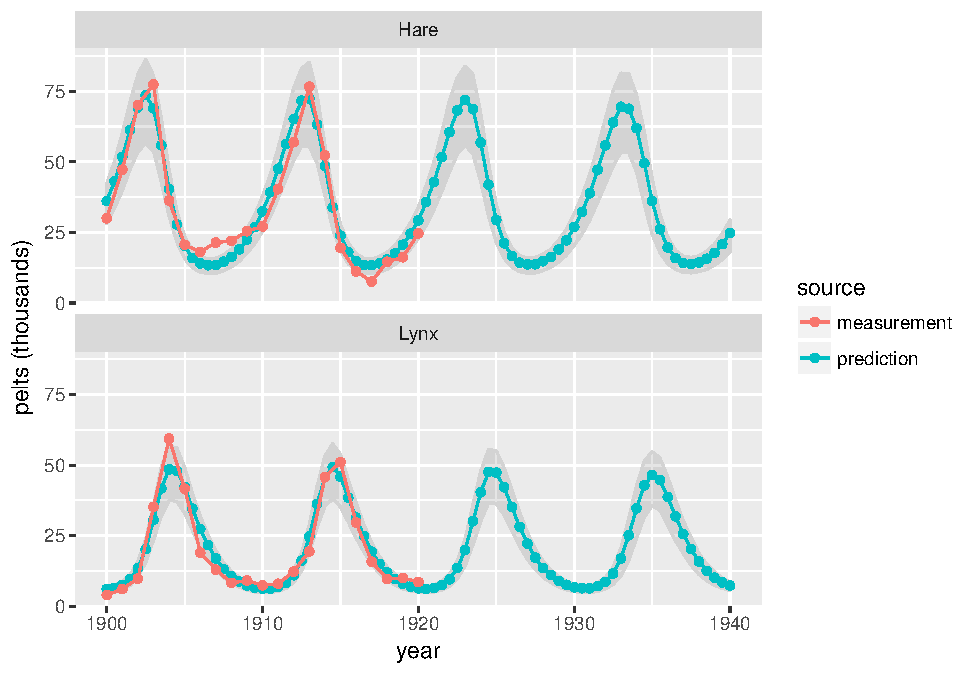
\includegraphics[width=0.8\textwidth]{img/lotka-volterra-predict.pdf}
\vspace*{-4pt}
\begin{subsubitemize}
\item training data (1900-1920); \ future predictions (1921+)
\end{subsubitemize}


\mypart{}{Bayesian Methodology}


\sld{Probability is Epistemic}
%
\begin{itemize}
\item \myemph{John Stuart Mill} ({\slshape Logic} 1882, Part III, Ch. 2):
\begin{subitemize}
\item ... the probability of an event is not a quality of the event itself, but a mere name for the degree of ground which we, or some one else, have for expecting it.
\item Every event is \myemph{in itself certain}, not probable; if we knew all, we should either know positively that it will happen, or positively that it will not.
\item ... its probability to us means the \myemph{degree of expectation of its occurrence}, which we are warranted in entertaining by our present evidence.
\end{subitemize}
\item Probabilities \myemph{quantify uncertainty}
\item Statistical reasoning is \myemph{counterfactual}
\end{itemize}


\sld{Random Variables}
%
\begin{itemize}
\item Random variables are the currency of probability theory
\item Random variables typically take numbers as values
\item Imagine a bin filled with balls representing the way the world might be
\item A ball records the value of every random variable
\item Examples
\begin{subitemize}
\item the sum of the three best among a roll of four dice (d6)
\item time before the next traffic accident on a given highway
\item prevalence of a disease in a population
\end{subitemize}
\end{itemize}


\sld{Events}
%
\begin{itemize}
\item Event is a set of outcomes
\item Usually subset of random variable values
\begin{subitemize}
\item prevalence of disease $\lambda > 0.02$
\item probability that one player is better than another, $\theta_1 >
  \theta_2$
\item probability that team A wins a game against B
\item probability that team A betas team B by more than 5 points
\end{subitemize}
\item Probability is that one of the outcomes occurs
\end{itemize}


\sld{Conditional Probability}
%
\begin{itemize}
\item What is probability a man is taller than 6'?
\begin{subitemize}
\item What if I tell you he's Dutch?
\item What if I tell you he's a professional athlete?
\item What if I tell you he's a jockey?  or basketball player?
\item What if I tell you his mother is taller than 6'?
\end{subitemize}
\end{itemize}


\sld{Bayesian Data Analysis}
%
\begin{itemize}
\item ``By {Bayesian data analysis}, we mean {practical methods}
  for making {inferences} from {data} using {probability models}
  for quantities we {observe} and about which we {wish to learn}.''
  %
\item ``The essential characteristic of Bayesian methods is
  their \myemph{explicit use of probability for quantifying uncertainty}
  in inferences based on statistical analysis.''
\end{itemize}
%
\vfill\hfill{\footnotesize Gelman et al., {\slshape Bayesian Data Analysis},
  3rd edition, 2013}


\sld{Bayesian Methodology}
%
\begin{itemize}
\item Set up \myemph{full probability model}
  \vspace*{-4pt}
  \begin{itemize}
  \item for \myemph{all} observable \& unobservable quantities
  \item consistent w. problem knowledge \& data collection
  \end{itemize}
  %
\item \myemph{Condition} on observed data (where Stan comes in!)
  \vspace*{-4pt}
  \begin{itemize}
  \item to calculate posterior probability of unobserved quantities
    (e.g., parameters, predictions, missing data)
  \end{itemize}
  %
\item \myemph{Evaluate}
  \vspace*{-4pt}
  \begin{itemize}
  \item model fit and implications of posterior
  \end{itemize}
\vfill
\item \myemph{Repeat} as necessary
\end{itemize}
\vfill\hfill {\footnotesize {\slshape Ibid.}}


\sld{Where do Models Come from?}
%
\begin{itemize}
\item Sometimes model comes first, based on substantive
  considerations
\begin{subitemize}
\item toxicology, economics, ecology, physics, \ldots
\end{subitemize}
\item Sometimes model chosen based on data collection
\begin{subitemize}
\item  traditional statistics of surveys and experiments
\end{subitemize}
\item Other times the data comes first
\begin{subitemize}
\item observational studies, meta-analysis, \ldots
\end{subitemize}
\hfill
\item Usually its a mix
\end{itemize}


\sld{Model Checking}
%
\begin{itemize}
\item Do the inferences make sense?
\begin{subitemize}
\item are parameter values consistent with model's prior?
\item does simulating from parameter values produce reasonable fake
  data?
\item are marginal predictions consistent with the data?
\end{subitemize}
\item Do predictions and event probabilities for new data make sense?
\vfill
\item {\slshape \myemph{Not}}: Is the model true?
\item {\slshape \myemph{Not}}: What is Pr[model is true]?
\item {\slshape \myemph{Not}}: Can we ``reject'' the model?
\end{itemize}


\sld{Model Improvement}
%
\begin{itemize}
\item Expanding the model
\begin{subitemize}
\item hierarchical and multilevel structure \ldots
\item more flexible distributions (overdispersion, covariance)
\item more structure (geospatial, time series)
\item more modeling of measurement methods and errors
\item \ldots
\end{subitemize}
\item Including more data
\begin{subitemize}
\item breadth (more predictors or kinds of observations)
\item depth (more observations)
\end{subitemize}
\end{itemize}


\sld{Properties of Bayesian Inference}
%
\begin{itemize}
\item Explores full range of parameters consistent with prior info and
  data$^*$
\begin{subitemize}
\item $^*$ if such agreement is possible
\item Stan automates this procedure with diagnostics
\end{subitemize}
\item Inferences can be plugged in directly for
\begin{subitemize}
\item parameter estimates minimizing expected error
\item predictions for future outcomes with uncertainty
\item event probability updates conditioned on data
\item risk assessment / decision analysis conditioned on uncertainty
\end{subitemize}
\end{itemize}


\sld{``All Models are Wrong,\\[8pt]\spc but some are useful''}
%
\begin{quote}
  \hspace*{-5pt}{\Large``}Now it would be very remarkable if any system existing in the real
  world could be exactly represented by any simple model. However,
  cunningly chosen parsimonious models often do provide remarkably
  useful approximations.{\Large''}
\\
\mbox{ } \hfill {\small --- George Box (1979)}

\end{quote}
\begin{itemize}
\item Slide title was section title in Box's paper
\end{itemize}
\vfill
\hfill {\tiny Box, G. E. P. 1979. Robustness in the strategy of
  scientific model building.  In
  {\slshape Robustness in Statistics}, Academic Press.}


\sld{Model (Mis)Specification}
%
\begin{itemize}
\item A model is \myemph{well specified} if it matches the data-generating
  process of the data.
\item All of our models will be \myemph{misspecified} to some extent
\begin{subitemize}
\item mildly misspecified: Newtonian physics (most speeds)
\item wildly misspecified: social science regression
\item wildly mispsecified: Newtonian physics (near speed of light)
\end{subitemize}
\item Models assumptions and predictions must be \myemph{tested}
\begin{subitemize}
\item ideally with \myemph{cross-validation} on quantities of interest
\end{subitemize}
\end{itemize}


\sld{The Folk Theorem}
%
\begin{quote}
\hspace*{-5pt}{\Large``}When you have computational problems, often there's a
problem with your model.{\Large''}
\\[4pt]
\mbox{ } \hfill {\small --- Andrew Gelman, blog}
\end{quote}
\begin{itemize}
\item The usual culprits are
\begin{subitemize}
\item bugs in: samplers, data munging, model coding, etc.
\item model misspecification
\end{subitemize}
\end{itemize}
\vfill
\hfill
{\footnotesize \url{http://andrewgelman.com/2008/05/13/the_folk_theore/}}


\sld{Model Calibration}
%
\begin{itemize}
\item Consider 100 days for which a meteorologist predicted a 70\%
  chance of rain
\begin{subitemize}
\item about 70 of them should have had rain
\item not fewer, not more!
\item technically, expect $\mathsf{Binomial}(100, 0.7)$ rainy day from
  a calibrated model
\end{subitemize}
\item Use posterior predictive checks to test calibration on
\begin{subitemize}
\item training data---can it fit?
\item held out data---can it predict?
\item cross-validation---approximates held out with trainin data
\end{subitemize}
\item Also applies to interval coverage of parameter values
\end{itemize}

\sld{Model Sharpness}
%
\begin{itemize}
\item Ideal forecasts are deterministic
\begin{subitemize}
\item predict 100\% chance of rain or 0\% chance of rain
\item always right
\end{subitemize}
%
\item A forecast of 90\% chance of rain reduces uncertainty more than a 50\% prediction
\item A model is \myemph{sharp} if it has narrow posterior intervals
\begin{subitemize}
\item Prediction $\mbox{Pr}[\alpha \in (1.2, 1.9)] = 0.9$
\item is sharper than $\mbox{Pr}[\alpha \in (1, 2)] = 0.9$
\end{subitemize}
\item I.e., sharper models are more certain in its predictions
\item Given calibration, we want our predictions to be \myemph{sharp}
\end{itemize}


\sld{Cross-Validation}
%
\begin{itemize}
\item Uses single data set to model held-out performance
\item Assumes stationarity (as most models do)
\item Partition data evenly into disjoint subsets (called \myemph{folds})
\begin{subitemize}
\item 10 is a common choice
\item \myemph{leave-one-out} (LOO) uses a the number of training
  data points
\end{subitemize}
\item For each fold
\begin{subitemize}
\item estimate model on all data but that fold
\item test on that fold
\end{subitemize}
\item Usual comparison statistic is held out log likelihood
\end{itemize}



\mypart{}{Bayesian Inference}


\sld{Notation for Basic Quantities}
%
\begin{itemize}
\item \myemph{Basic Quantities}
\begin{subitemize}
\item $y$: \ observed data
\item $\theta$: \ parameters (and other unobserved quantities)
\item $x$: \ constants, predictors for conditional (aka ``discriminative'') models
\end{subitemize}
\item \myemph{Basic Predictive Quantities}
\begin{subitemize}
\item $\tilde{y}$: unknown, potentially observable quantities
\item $\tilde{x}$: \ constants, predictors for unknown quantities
\end{subitemize}
\end{itemize}


\sld{Naming Conventions}
%
\begin{itemize}
\item \myemph{Joint}: \ $p(y,\theta)$
\item \myemph{Sampling / Likelihood}: \ $p(y|\theta)$
\begin{subitemize}
\item Sampling is function of $y$ with $\theta$ fixed (prob function)
\item Likelihood is function of $\theta$ with $y$ fixed (\emph{not} prob function)
\end{subitemize}
\item \myemph{Prior}: \ $p(\theta)$
\item \myemph{Posterior}: \ $p(\theta|y)$
\item \myemph{Data Marginal (Evidence)}: \ $p(y)$
\item \myemph{Posterior Predictive}: \ $p(\tilde{y}|y)$
\end{itemize}


\sld{Bayes's Rule for Posterior}
%
\vspace*{-4pt}
\begin{eqnarray*}
    p(\theta|y)
    & = & \frac{p(y,\theta)}{p(y)}
          \hspace*{64pt} \text{\small [def of conditional]}
    \\[6pt]
    & = & \frac{p(y|\theta) \, p(\theta)}{p(y)}
          \hspace*{44pt} \text{\small [chain rule]}
    \\[6pt]
    & = & \frac{p(y|\theta) \, p(\theta)}{\int_{\Theta} p(y,\theta') \ d\theta'}
          \hspace*{40pt} \text{\small [law of total prob]}
    \\[6pt]
    & = & \frac{p(y|\theta) \, p(\theta)}{\int_{\Theta} p(y|\theta') \,
      p(\theta') \ d\theta'}
          \hspace*{20pt} \text{\small [chain rule]}
\end{eqnarray*}
\vfill
\begin{itemize}
\item \emph{Inversion:} Final result depends only on
  sampling distribution (likelihood) $p(y|\theta)$ and prior
  $p(\theta)$
\end{itemize}


\sld{Bayes's Rule up to Proportion}
%
\begin{itemize}
\item If data $y$ is fixed, then
\begin{eqnarray*}
p(\theta|y)
& = & \frac{p(y|\theta) \, p(\theta)}{p(y)}
\\[6pt]
& \propto & p(y|\theta) \, p(\theta)
\\[6pt]
& = & p(y,\theta)
\end{eqnarray*}
\item Posterior proportional to likelihood times prior
\item Equivalently, posterior proportional to joint
\vfill
\item The nasty integral for data marginal $p(y)$ goes away
\end{itemize}

\mypart{}{What Stan Computes}

\sld{Draws from Posterior}
%
\begin{itemize}
\item Stan performs (Markov chain) Monte Carlo sampling
\item Produces sequence of draws
\[
\theta^{(1)}, \theta^{(2)}, \ldots, \theta^{(M)}
\]
\item wher each draw $\theta^{(m)}$ is marginally distributed according to the posterior
$p(\theta | y)$
\item Draws characterize posterior
\item Plot with histograms, kernel density estimates, etc.
\end{itemize}

\sld{Parameter Estimates}
%
\begin{itemize}
\item An estimator maps data into a parameter estimate
\item The standard Bayesian estimator is the posterior mean
\begin{eqnarray*}
\hat{\theta}
& = &
\mathbb{E}[\theta \mid y]
\\[6pt]
& = &
 \int_{\Theta} \ \theta \ p(\theta | y) \ \mathrm{d}\theta
\\[6pt]
& \approx &
\frac{1}{M} \sum_{m=1}^M \theta^{(m)}
\end{eqnarray*}
\item Posterior mean minimizes expected square error
\[
\hat{\theta} = \mbox{arg min}_{\theta} \mathbb{E}[(\theta -
\hat{\theta})^2]
\]
\end{itemize}


\sld{Parameter Variance Estimates}
%
\begin{itemize}
\item Variances is expected squared error
\item Calculated by plugging in estimated value $\hat{\theta}$
\begin{eqnarray*}
\mathrm{var}[\theta \mid y]
& = & \mathbb{E}[(\theta - \mathbb{E}[\theta \mid y])^2 \mid y]
\\[6pt]
& = & \int (\theta - \hat{\theta})^2 \, p(\theta | y) \, \mathrm{d}\theta
\\[6pt]
& \approx &
\frac{1}{M - 1} \sum_{m=1}^M (\theta^{(m)} - \hat{\theta})^2
\end{eqnarray*}
\end{itemize}


\sld{Posterior Quantiles}
%
\begin{itemize}
\item Let $Y$ be a random variable
\item If $\mbox{Pr}[Y \leq q] = \alpha$, then $q$ is the
  $\alpha$-quantile of $Y$
\item Median is 0.5 quantile, i.e., $q$ such that $\mbox{Pr}[Y \leq q] = 0.5$
\item Central 90% interval spans from quantile 0.05 to quantile 0.95
\item To compute quantile $\alpha$ for $\theta$ in the posterior
  $p(\theta | y)$:
\[
\mathrm{quantile}(\theta, \alpha)
\ = \
\mathrm{sort\_ascending}(\theta^{(1)}, \ldots, \theta^{(M)})
\left[ \, \lceil \alpha \times M \rceil \, \right]
\]
\end{itemize}


\sld{Event Probabilities}
%
\begin{itemize}
\item Events are fundamental probability bearing units which
\begin{subitemize}
\item are defined by sets of outcomes
\item which occur or not with some probability
\end{subitemize}
\item Outcomes defined by values of random variables
\item Use conditions on parameters to define sets of outcomes
\begin{subitemize}
\item e.g., $\theta_b > \theta_g$ for more boy births than girl births
\item e.g., $z_k = 1$ for team A beating team B in game $k$
\end{subitemize}
\item A set $S$ corresponds to an indicator function $f$,
\[
f(s) =
\begin{cases}
1 & \mbox{if } s \in S
\\
0 & \mbox{if } s \not\in S
\end{cases}
\]
\end{itemize}


\sld{Calculating Event Probabilities}
%
\begin{itemize}
\item Event probabilities are expectations of indicator functions
\item Write the indicator function for event $E$ be $\mbox{cond}(\theta)$
%
\begin{eqnarray*}
\mbox{Pr}[E \mid y]
& = & \mathbb{E}[\mbox{cond}(\theta) \mid y]
\\[6pt]
& = & \int_{\Theta} \mathrm{I}[\mbox{cond}(\theta) \mid y] \, \mathrm{d}\theta
\\[6pt]
& \approx &
\frac{1}{M} \sum_{m=1}^M \mathrm{I}[\mbox{cond}(\theta^{(m)})]
\end{eqnarray*}
%
\item Just proportion of posterior draws for which condition holds
\end{itemize}


\sld{Posterior Event Probabilities}
%
\begin{itemize}
\item An \myemph{event} $A$ is a collection of outcomes
\item So $A$ may be defined by an indicator $f$ on parameters
\[
f(\theta)
=
\begin{cases}
1 & \text{if } \theta \in A
\\
0 & \text{if } \theta \not\in A
\end{cases}
\]
\begin{subitemize}
\item $f(\theta) = \mathrm{I}(\theta_1 > \theta_2)$
\ \ for \ \ $\Prob{\theta_1 > \theta_2 \, | \, y}$,
\item $f(\theta) = \mathrm{I}(\theta \in (0.50, 0.52)$ for $\mathrm{Pr}\left[ \theta \in (0.50, 0.52) \,|\, y \right]$
\end{subitemize}
\item Defined by posterior expectation of indicator $f(\theta)$
\[
\mathrm{Pr}[A \,|\, y]
\ = \
\mathbb{E}\left[ f(\theta) \, | \, y \right]
\ = \
\int_{\Theta} f(\theta) \, p(\theta|y) \, d\theta.
\]
\end{itemize}


\sld{Posterior Predictive Distribution}
%
\begin{itemize}
\item Predict new data $\tilde{y}$ based on observed data $y$
\item Marginalize parameters $\theta$ out of posterior and likelihood
\begin{eqnarray*}
p(\tilde{y} \mid y)
& = & \mathbb{E}[p(\tilde{y} | \theta) \mid y]
\\[6pt]
& = &
\int p(\tilde{y} | \theta) \, p(\theta | y) \, \mathrm{d}\theta.
\\[6pt]
& \approx &
\frac{1}{M} \sum_{m=1}^M p(\tilde{y} | \theta^{(m)})
\end{eqnarray*}
\item Weights predictions $p(\tilde{y}|\theta)$ by posterior $p(\theta|y)$
\end{itemize}





\sld{Calculations in Stan}
%
\begin{itemize}
\item Stan automatically computes estimates, variances, and quantiles
  for parameters
\item To compute event probabilities, define indicator in generated
  quantities block
\begin{stancode}
generated quantities {
  int<lower=0, upper=1> theta_gt_half = (theta > 0.5);
}
\end{stancode}
\item To compute predictions, define with random number generators in
  the generated quantities block
\begin{stancode}
generated quantities {
  real y_predict = normal_rng(x_predict * alpha, sigma);
}
\end{stancode}
\end{itemize}


\mypart{}{Repeated Binary Trials}


\sld{Repeated Binary Trial Model}
%
\begin{itemize}
%
\vspace*{-4pt}
\item \myemph{Data}
\begin{subitemize}
  \item $N \in \setcomp{0, 1, \ldots}$: number of trials (constant)
  \item $y_n \in \setcomp{0, 1}$: trial $n$ success (known, modeled data)
\end{subitemize}
%
\vspace*{-6pt}
\item \myemph{Parameter}
\begin{subitemize}
\item $\theta \in [0, 1]$ : chance of success (unknown)
\end{subitemize}
%
\vspace*{-6pt}
\item \myemph{Prior}
\begin{subitemize}
\item $p(\theta)
\ = \
\distro{Uniform}(\theta \,|\, 0, 1) = 1$
\end{subitemize}
%
\vspace*{-6pt}
\item \myemph{Likelihood}
\begin{subitemize}
\item $p(y \,|\, \theta)
\ = \ \prod_{n=1}^N \distro{Bernoulli}(y_n \,|\, \theta)
\ = \ \prod_{n=1}^N \theta^{y_n} \, (1 - \theta)^{1 - y_n}$
\end{subitemize}
%
\vspace*{-6pt}
\item \myemph{Posterior}
\begin{subitemize}
\item
$p(\theta \, | \, y)
\propto
p(\theta) \, p(y \, | \, \theta)$
\end{subitemize}
\end{itemize}



\sld{Stan Program}
%
\begin{stancode}
data {
  int<lower=0> N;                 // number of trials
  int<lower=0, upper=1> y[N];     // success on trial n
}
parameters {
  real<lower=0, upper=1> theta;   // chance of success
}
model {
  theta ~ uniform(0, 1);          // prior
  y ~ bernoulli(theta);           // likelihood
}
\end{stancode}


\sld{A Stan Program...}
%
\begin{itemize}
\item defines log (posterior) density up to constant, so...
\item equivalent to define log density directly:
\begin{stancode}
model {
  target += 0;
  for (n in 1:N)
    target += log(y[n] ? theta : (1 - theta));
}
\end{stancode}
\item equivalent to drop constant prior and vectorize
  likelihood:
\begin{stancode}
model {
  y ~ bernoulli(theta);
}
\end{stancode}
\end{itemize}


\sld{R: Simulate Data}
%
\begin{itemize}
\item Generate data
\begin{codein}
> theta <- 0.30;
> N <- 20;
> y <- rbinom(N, 1, 0.3);

> y
\end{codein}
\begin{codeout}
 [1] 1 1 1 1 0 0 0 0 1 1 0 0 1 0 0 0 0 0 0 1
\end{codeout}
\item Calculate MLE as sample mean from data
\begin{codein}
> sum(y) / N
\end{codein}
\begin{codeout}
[1] 0.4
\end{codeout}
\end{itemize}


\sld{RStan: Bayesian Posterior}
%
\begin{codein}
> library(rstan);

> fit <- stan("bern.stan",
              data = list(y = y, N = N));

> print(fit, probs=c(0.1, 0.9));
\end{codein}
\begin{codeout}
Inference for Stan model: bern.
4 chains, each with iter=2000; warmup=1000; thin=1;
post-warmup draws per chain=1000,
total post-warmup draws=4000.

        mean se_mean   sd    10%    90% n_eff Rhat
theta   0.41    0.00 0.10   0.28   0.55  1580    1
\end{codeout}


\sld{Plug in Posterior Draws}
%
\begin{itemize}
\item Extracting the posterior draws
\begin{codein}
> theta_draws <- extract(fit)$theta;
\end{codein}
\item Calculating posterior mean (estimator)
\begin{codein}
> mean(theta_draws);
\end{codein}
\begin{codeout}
[1] 0.4128373
\end{codeout}
\item Calculating posterior intervals
\begin{codein}
> quantile(theta_draws, probs=c(0.10, 0.90));
\end{codein}
\begin{codeout}
      10%       90%
0.2830349 0.5496858
\end{codeout}
\end{itemize}




\sld{Marginal Posterior Histograms}
%
\begin{codein}
theta_draws_df <- data.frame(list(theta = theta_draws));
plot <-
  ggplot(theta_draws_df, aes(x = theta)) +
  geom_histogram(bins=20, color = "gray");
plot;
\end{codein}
\vspace*{-9pt}
\begin{center}
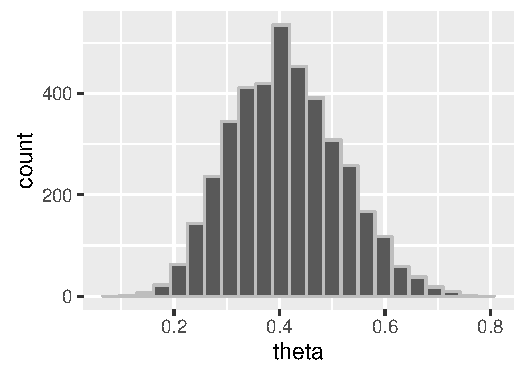
\includegraphics[height=1.25in]{img/bern-posterior-histogram.pdf}
\end{center}
\vspace*{-0.1in}
\begin{subitemize}
\item
Displays the full posterior {\slshape marginal} distribution $p(\theta \,
| \, y)$
\end{subitemize}



\sld{RStan: MAP, penalized MLE}
%
\begin{itemize}
\item Stan's optimization for estimation; two views:
\begin{subitemize}
\item max posterior mode, aka max a posteriori (MAP)
\item max penalized likelihood (MLE)
\end{subitemize}
\end{itemize}
\vspace*{-6pt}
\begin{stancode}
> library(rstan);
> N <- 5;
> y <- c(0,1,1,0,0);
> model <- stan_model("bernoulli.stan");
> mle <- optimizing(model, data=c("N", "y"));
...
> print(mle, digits=2)
$par              $value  (log density)
theta             [1] -3.4
  0.4
\end{stancode}
% \begin{subitemize}
% \item Posterior: $\distro{Beta}(1+2, 1+3)$;  mode $0.40$; mean $0.43$
% \item Density: MLE w/o Jacobian;  MCMC with Jacobian
% \end{subitemize}



\mypart{}{Male Birth Ratio}


\sld{Birth Rate by Sex}
\begin{itemize}
\item \myemph{Laplace}'s data on live births in Paris from 1745--1770:
\vspace*{-4pt}
\begin{center}\small
\begin{tabular}{c|c}
{\slshape sex} & {\slshape live births}
\\ \hline
female & 241\,945
\\
male & 251\,527
\end{tabular}
\end{center}
\item \myemph{Question 1} (Estimation)
\\
What is the birth rate of boys vs. girls?

\item \myemph{Question 2} (Event Probability)
\\
Is a boy more likely to be born than a girl?
%
\item Bayes (1763) set up the ``Bayesian'' model
\item Laplace (1781, 1786) solved for the posterior
\end{itemize}


\sld{Binomial Distribution}
%
\begin{itemize}
\item Binomial distribution is number of successes $y$ in $N$
i.i.d. Bernoulli trials with chance of success $\theta$
\item If $y_1,\ldots,y_N\sim \distro{Bernoulli}(\theta)$,
\\[4pt] then $(y_1 + \cdots + y_N) \sim \distro{Binomial}(N,\theta)$
\item The analytic form is
\[
\distro{Binomial}(y|N,\theta)
\ = \ \binom{N}{y} \theta^{y} (1 - \theta)^{N-y}
\]
where the binomial coefficient normalizes for permutations (i.e.,
which subset of $n$ has $y_n = 1$),
\[
\binom{N}{y} = \frac{N!}{y! \, (N-y)!}
\]
\end{itemize}


\sld{Mathematics vs.\ Simulation}
%
\begin{itemize}
\item Luckily, we don't have to be as good at math as Laplace
\item Nowadays, we calculate all these integrals by computer using
  tools like Stan
\vfill
\begin{quote}
  If you wanted to do foundational research in statistics in the
  mid-twentieth century, you had to be bit of a mathematician, whether
  you wanted to or not. \ldots if you want to do statistical research
  at the turn of the twenty-first century, you have to be a computer
  programmer.  \\[3pt] \mbox{ } \hfill {--- Andrew Gelman (2009)}
\end{quote}
\vfill
{\tiny Gelman. 2009. Bayes, Jeffreys, Prior Distributions and
the Philosophy of Statistics. {\slshape Statistical Science} 24(2).
\end{itemize}


\sld{Bayes's Binomial Model}
%
\begin{itemize}
\item{Data}
\begin{subitemize}
\item $y$: total number of male live births (251,527)
\item $N$ : total number of live births (493,472)
\end{subitemize}
\item Parameter
\begin{subitemize}
\item $\theta \in (0,1)$: proportion of male live births
\end{subitemize}
\item Likelihood
\[
p(y|N,\theta)
\ = \ \distro{Binomial}(y|N,\theta)
\ = \ \binom{N}{y} \theta^{y} (1 - \theta)^{N-y}
\]
\item Prior
\[
p(\theta)
\ = \ \distro{Uniform}(\theta \, | \, 0,1)
\ = \ 1
\]
\end{itemize}


\sld{Laplace Turns the Crank}
%
\begin{itemize}
\item Given Bayes's general formula for the posterior
\[
p(\theta|y,N)
\ = \
\frac{\distro{Binomial}(y|N,\theta) \, \distro{Uniform}(\theta|0,1)}
     {\int_{\Theta} \distro{Binomial}(y|N,\theta') \,  p(\theta')
       d\theta'}
\]
\item Laplace used Euler's Beta function (B) to normalize the
  posterior, with final solution
\[
p(\theta|y,N)
\ = \ \distro{Beta}(\theta \, | \, y + 1, \ N - y + 1)
\]
\end{itemize}


\sld{Laplace turns the Crank}
%
\begin{itemize}
\item What is probability that a male live birth is more probable?
\begin{eqnarray*}
\Prob{\theta > 0.5}
& = &  \int_{\Theta} \indicator{\theta > 0.5} \, p(\theta|y,N) d\theta
\\[4pt]
& = &  \int_{0.5}^1 p(\theta|y,N) d\theta
\\[4pt]
& \approx &  1 - 10^{-42}
\end{eqnarray*}
\item  Laplace solved Bayes's integral by
\begin{subitemize}
\item determining that the posterior was a beta distribution (conjugacy!)
\item and solving the normalization (gamma functions)
\end{subitemize}
\end{itemize}


\sld{Beta Distribution}
%
\begin{itemize}
\item Required for analytic posterior of Bayes's model
\item For parameters $\alpha,\beta > 0$ and $\theta \in (0,1)$,
\[
\distro{Beta}(\theta|\alpha,\beta)
\ = \ \frac{1}{\Betafun(\alpha,\beta)}
      \theta^{\alpha - 1} \,
      (1 - \theta)^{\beta-1}
\]
\item Euler's Beta function is used to normalize,
\[
\Betafun(\alpha,\beta)
\ = \ \int_0^1 u^{\alpha-1}(1-u)^{\beta-1} du
\ = \ \frac{\Gamma(\alpha)\,\Gamma(\beta)}{\Gamma(\alpha + \beta)}
\]
where $\Gamma()$ is continuous generalization of factorial
\item Note: \ $\distro{Beta}(\theta|1,1) = \distro{Uniform}(\theta|0,1)$
\end{itemize}


\sld{Beta Distribution --- Examples}
%
\vspace*{-4pt}
\begin{itemize}
\item Unnormalized posterior density assuming uniform prior and $y$
  successes out of $n$ trials (all with mean 0.6).
\end{itemize}
\begin{center}
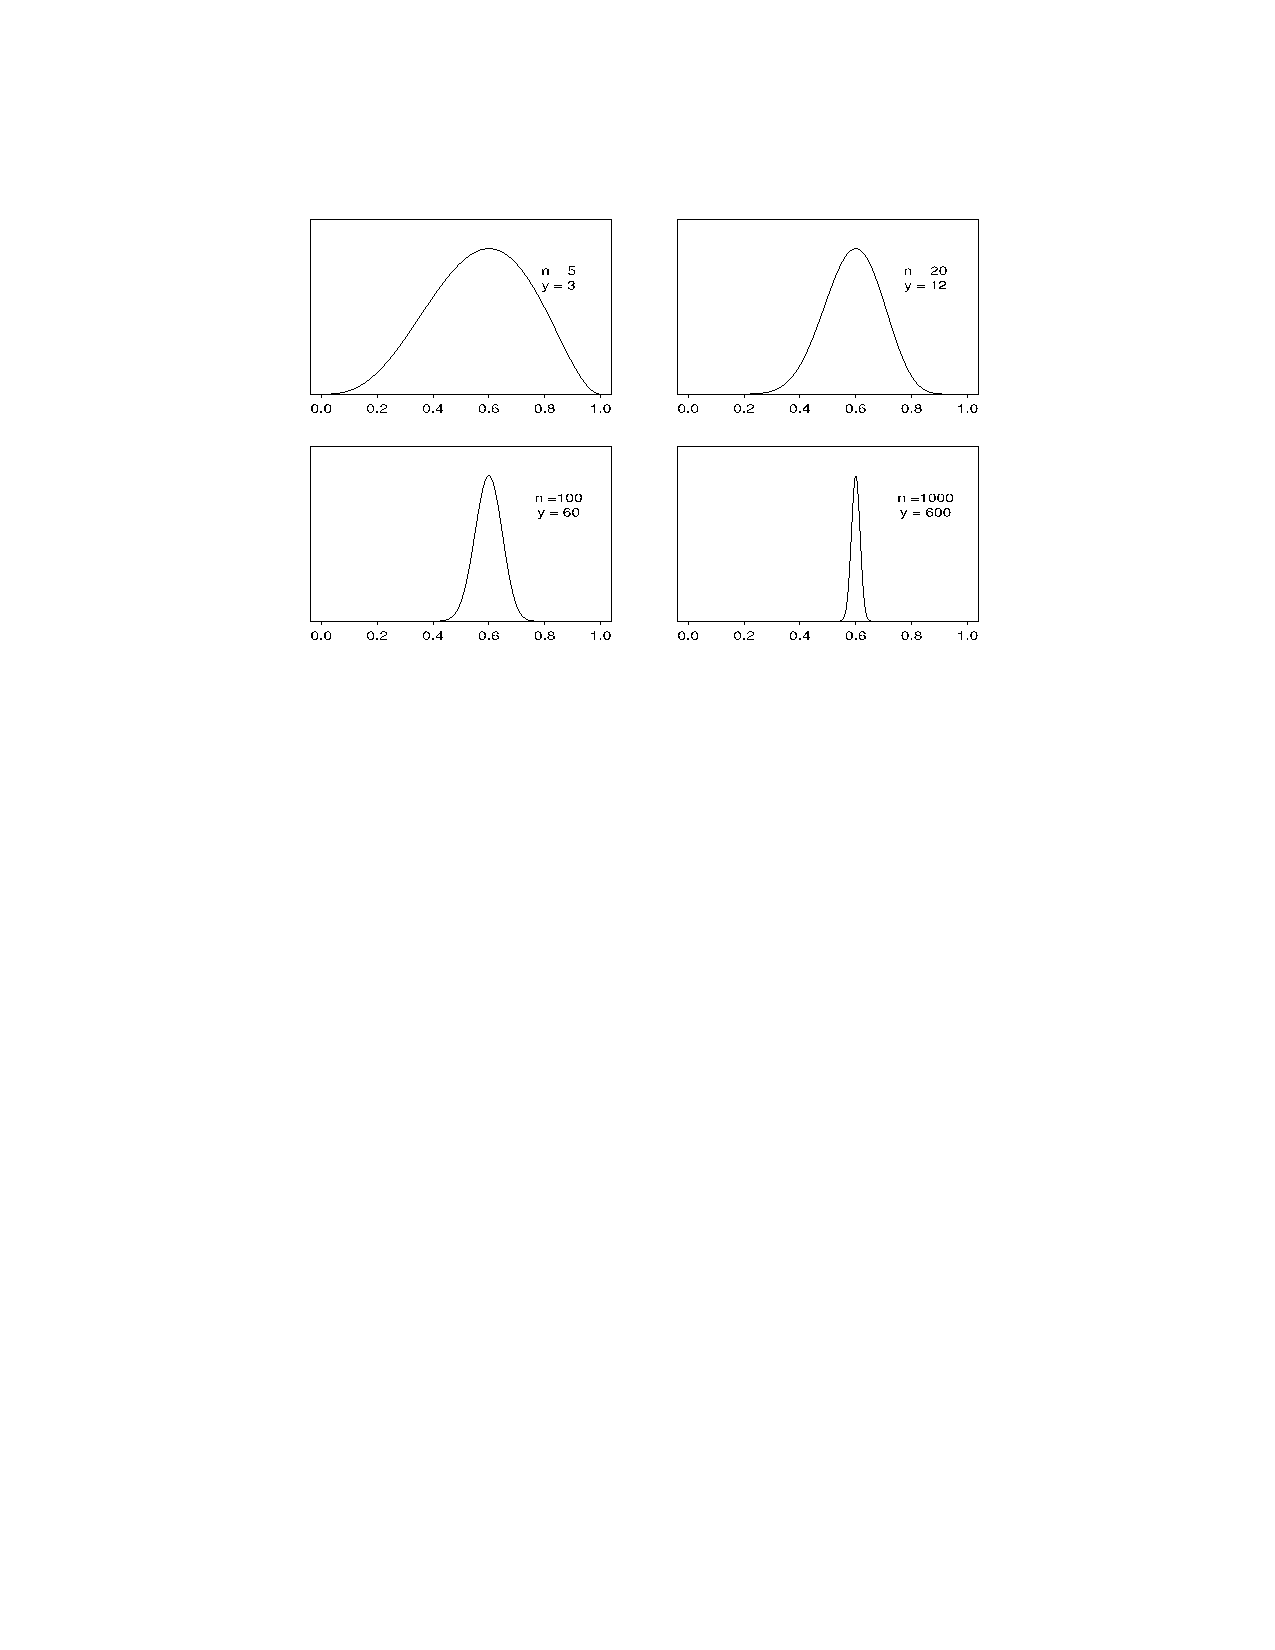
\includegraphics[height=1.6in]{img/bda-beta-plots.pdf}
\end{center}
\vspace*{-12pt}
\hfill {\tiny Gelman et al. (2013) {\slshape Bayesian Data Analysis},
  3rd Edition.}


\sld{Replacing Laplace with Stan}
%
\begin{stancode}
transformed data {
  int male = 251527;
  int female = 241945;
}
parameters {
  real<lower=0, upper=1> theta;
}
model {
  male ~ binomial(male + female, theta);
}
generated quantities {
  int<lower=0, upper=1> theta_gt_half = (theta > 0.5);
}
\end{stancode}


\sld{And the Answer is...}
%
\begin{codein}
> fit <- stan("laplace.stan", iter=100000);
> print(fit, probs=c(0.005, 0.995), digits=3)
\end{codein}
\begin{codeout}
                    mean   0.5%  99.5%
theta               0.51  0.508  0.512
theta_gt_half       1.00  1.000  1.000
\end{codeout}
%
\begin{itemize}
\item Q1: $\theta$ is 99\% certain to lie in $(0.508, 0.512)$
%
\item Q2:  Laplace ``morally certain'' boys more prevalent
\end{itemize}


\sld{Estimation}
%
\begin{itemize}
\item Posterior is $\distro{Beta}(\theta \, | \, 1 + 241\,945, \ 1 + 251\,527)$
\item Posterior mean:
\[
\frac{1 + 251\,527}
     {1 + 241\,945 + 1 + 251\,527}
\approx 0.5097087{\bf3}
\]
\item Maximum likelihood estimate same as posterior mode (because
  of uniform prior)
\[
\frac{251\,527}
     {241\,945 + 251\,527}
\approx 0.5097088{\bf2}
\]
\item As number of observations approaches $\infty$,
\\
MLE approaches posterior mean
\end{itemize}


\sld{Event Probability Inference}
%
\begin{itemize}
\item What is probability that a male live birth is more likely than a
  female live birth?
\begin{eqnarray*}
\Prob{\theta > 0.5}
& = &  \int_{\Theta} \indicator{\theta > 0.5} \, p(\theta|y,N) d\theta
\\[4pt]
& = &  \int_{0.5}^1 p(\theta|y,N) d\theta
\\[4pt]
& = &  1 - F_{\theta|y,N}(0.5)
\\[4pt]
& \approx &  10^{-42}
\end{eqnarray*}
\item $\indicator{\phi} = 1$ if condition $\phi$ is true and 0 otherwise.
\item  $F_{\theta|y,N}$ is posterior cumulative distribution
function (cdf).
\end{itemize}



\mypart{}{Conjugate Priors}


\sld{Conjugate Priors}
%
\begin{itemize}
\item Family $\mathcal{F}$ is a conjugate prior for family
  $\mathcal{G}$ if
\begin{subitemize}
\item prior in $\mathcal{F}$ and
\item likelihood in $\mathcal{G}$,
\item entails posterior in $\mathcal{F}$
\end{subitemize}
\item Before MCMC techniques became practical, Bayesian analysis
  mostly involved conjugate priors
\item Still widely used because analytic solutions are more efficient
  than MCMC
\end{itemize}

\sld{Beta is Conjugate to Binomial}
%
\vspace*{-2pt}
\begin{itemize}
\item Prior: \ \ \ \ \ \ \ \ \ \ \ $p(\theta|\alpha,\beta) =
  \distro{Beta}(\theta|\alpha,\beta)$
\item Likelihood: \ \ $p(y|N,\theta) = \distro{Binomial}(y|N,\theta)$
\item Posterior:
{\small
\begin{eqnarray*}
p(\theta|y,N,\alpha,\beta)
& \propto & p(\theta|\alpha,\beta) \, p(y|N,\theta)
\\[6pt]
& = & \distro{Beta}(\theta|\alpha,\beta)
      \, \distro{Binomial}(y|N,\theta)
\\
& = & \frac{1}{\Betafun(\alpha,\beta)}
      \theta^{\alpha - 1} \,
      (1 - \theta)^{\beta-1}
      \ \
      \binom{N}{y} \theta^{y} (1 - \theta)^{N-y}
\\[6pt]
& \propto &
      \theta^{y + \alpha - 1} \,
      (1 - \theta)^{N - y + \beta - 1}
\\[6pt]
& \propto & \distro{Beta}(\theta|\alpha + y, \ \beta + (N - y))
\end{eqnarray*}
}
\end{itemize}


\sld{Chaining Updates}
%
\vspace*{-4pt}
\begin{itemize}
\item Start with prior $\distro{Beta}(\theta|\alpha,\beta)$
\item Receive binomial data in $K$ stages $(y_1, N_1), \ldots, (y_K, N_K)$
\item After $(y_1,N_1)$, posterior is
  $\distro{Beta}(\theta|\alpha + y_1, \ \beta + N_1 - y_1)$
\item Use as prior for $(y_2,N_2)$, with posterior \\[3pt]
  $\distro{Beta}(\theta|\alpha + y_1 + y_2, \ \ \beta + (N_1 -
  y_1) + (N_2 - y_2))$
\item Lather, rinse, repeat, until final posterior
\[
\distro{Beta}(\theta|\alpha + y_1 + \cdots + y_K, \ \ \beta + (N_1 +
\cdots + N_K) - (y_1 + \cdots + y_K))
\]
\item Same result as if we'd updated with combined data \\[3pt]
$\distro{Beta}(y_1 + \cdots + y_K, \ \ N_1 + \cdots + N_K)$
\end{itemize}


\mypart{}{Fisher "Exact" Test}


\sld{Bayesian ``Fisher Exact Test''}
%
\vspace*{-4pt}
\begin{itemize}
\item Suppose we observe the following data on handedness
\begin{center}
{\small
\begin{tabular}{c|c|c||c}
     & {\slshape sinister} & {\slshape dexter} & TOTAL
\\ \hline \hline
{\slshape male} & 9 ($y_1$) & 43 & 52 ($N_1$)
\\
{\slshape female} & 4 ($y_2$) & 44 & 48 ($N_2$)
\end{tabular}
}
\end{center}
\item Assume likelihoods $\distro{Binomial}(y_k|N_k,\theta_k)$, uniform
  priors
\item Are men more likely to be lefthanded?
{\small
\begin{eqnarray*}
\Prob{\theta_1 > \theta_2 \, | \, y, N}
& = &
\int_{\Theta} \indicator{\theta_1 > \theta_2} \, p(\theta|y,N) \,
d\theta
\\[4pt]
& \approx & \frac{1}{M} \sum_{m=1}^M \indicator{\theta_1^{(m)} > \theta_2^{(m)}}.
\end{eqnarray*}
}
\end{itemize}


\sld{Stan Binomial Comparison}
%
\begin{stancode}
data {
  int y[2];
  int N[2];
}
parameters {
  vector<lower=0,upper=1> theta[2];
}
model {
  y ~ binomial(N, theta);
}
generated quantities {
  real boys_minus_girls = theta[1] - theta[2];
  int boys_gt_girls = theta[1] > theta[2];
}
\end{stancode}


\sld{Binomial Comparison Results}
%
\begin{codeout}
                   mean    2.5%  97.5%
theta[1]           0.22    0.12   0.35
theta[2]           0.11    0.04   0.21
boys_minus_girls   0.12   -0.03   0.26
boys_gt_girls      0.93    0.00   1.00
\end{codeout}
\begin{itemize}
\item
$\mathrm{Pr}[\theta_1 > \theta_2 \,|\, y] \approx 0.93$
\item
$\mathrm{Pr}\left[
(\theta_1 - \theta_2) \in (-0.03, 0.26)
\,|\, y
\right]
\, = \, 95\%$
\end{itemize}


\sld{Visualizing Posterior Difference}
%
\begin{itemize}
\item Plot of posterior difference, $p(\theta_1 - \theta_2 \, | \, y,
  N)$ (men - women)
\begin{center}
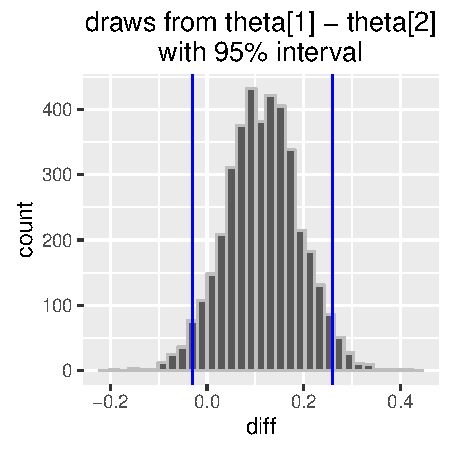
\includegraphics[height=1.65in]{img/lefty-posterior.pdf}
\end{center}
\item Vertical bars: central 95\% posterior interval $(-0.03,0.26)$
\end{itemize}


\mypart{}{More Stan Models}


\sld{Posterior Predictive Distribution}
%
\begin{itemize}
\item Predict new data ($\tilde{y}$) given observed data ($y$)
\item Includes two kinds of uncertainty
\begin{subitemize}
\item parameter estimation uncertainty: $p(\theta | y)$
\item sampling uncertainty:  $p(\tilde{y} | \theta)$
\end{subitemize}
\vspace*{-8pt}\begin{eqnarray*}
p(\tilde{y} |  y)
& = & \int p(\tilde{y} | \theta)
           \ p(\theta | y)
           \ \mathrm{d}\theta
\\[4pt]
& \approx & \frac{1}{M} \sum_{m=1}^M p(\tilde{y} | \theta^{(m)})
\end{eqnarray*}
\item Can generate predictions as sample of draws $\tilde{y}^{(m)}$
  based on $\theta^{(m)}$
\end{itemize}


\sld{Posterior Predictive Inference}
%
\begin{itemize}
\item Parameters $\theta$, observed data $y$, and data to predict $\tilde{y}$
\[
p(\tilde{y}|y) = \int_{\Theta} p(\tilde{y}|\theta) \ p(\theta|y) \ d\theta
\]
\item
{\small
\begin{Verbatim}
data {
  int<lower=0> N_tilde;
  matrix[N_tilde,K] x_tilde;
  ...
parameters {
  vector[N_tilde] y_tilde;
  ...
model {
  y_tilde ~ normal(x_tilde * beta, sigma);
\end{Verbatim}
}
\end{itemize}


\sld{Predict w.\ Generated Quantities}
%
\begin{itemize}
\item Replace sampling with pseudo-random number generation
\begin{stancode}
   generated quantities {
     vector[N_tilde] y_tilde;

     for (n in 1:N_tilde)
       y_tilde[n] = normal_rng(x_tilde[n] * beta, sigma);
   }
\end{stancode}
\item Must include noise for predictive uncertainty
\item PRNGs only allowed in generated quantities block
\begin{subitemize}
\item more computationally efficient per iteration
\item more statistically efficient with i.i.d.\ samples \\
(i.e., MC, not MCMC)
\end{subitemize}
\end{itemize}


\sld{Linear Regression with Prediction}
%
\begin{stancode}
data {
  int<lower=0> N;               int<lower=0> K;
  matrix[N, K] x;               vector[N] y;
  matrix[N_tilde, K] x_tilde;
}
parameters {
  vector[K] beta;               real<lower=0> sigma;
}
model {
  y ~ normal(x * beta, sigma);
}
generated quantities {
  vector[N_tilde] y_tilde
    = normal_rng(x_tilde * beta, sigma);
}
\end{stancode}


\sld{Transforming Precision to Scale}
%
\begin{stancode}
    parameters {
      real<lower=0> tau;
      ...
    }
    transformed parameters {
      real<lower=0> sigma = tau^(-0.5);
    }
\end{stancode}


\sld{Transform: Non-Centered Params}
%
\begin{stancode}
parameters {
  vector[K] beta_std;  // non-centered
}
transformed parameters {
  vector[K] beta =  mu + sigma * beta_std;
}
model {
  // implies:  beta ~ normal(mu, sigma)
  beta_std ~ normal(0, 1);
}
\end{stancode}


\sld{Logistic Regression}
%
\begin{stancode}
     data {
       int<lower=1> K;
       int<lower=0> N;
       matrix[N,K] x;
       int<lower=0,upper=1> y[N];
     }
     parameters {
       vector[K] beta;
     }
     model {
        beta ~ cauchy(0, 2.5);          // prior
        y ~ bernoulli_logit(x * beta);  // likelihood
     }
\end{stancode}


\sld{Generalized Linear Models}
%
\begin{itemize}
\item Direct parameterizations more efficient and stable
\item \myemph{Logistic regression} (boolean/binary data)
\begin{subitemize}
\item \Verb|y ~ bernoulli(inv_logit(eta));|
\item \Verb|y ~ bernoulli_logit(eta);|
\item Probit via \code{Phi} (normal cdf)
\item Robit (robust) via Student-$t$ cdf
\end{subitemize}
\item \myemph{Poisson regression} (count data)
\begin{subitemize}
\item \Verb|y ~ poisson(exp(eta));|
\item \Verb|y ~ poisson_log(eta);|
\item Overdispersion with negative binomial
\end{subitemize}
\end{itemize}


\sld{GLMS, continued}
%
\begin{itemize}
\item \myemph{Multi-logit regression} (categorical data)
\begin{subitemize}
\item \Verb|y ~ categorical(softmax(eta));|
\item \Verb|y ~ categorical_logit(eta);|
\end{subitemize}
\item \myemph{Ordinal logistic regression} (ordered data)
\begin{subitemize}
\item Add cutpoints \code{c}
\item \Verb|y ~ ordered_logistic(eta, c);|
\end{subitemize}
\item \myemph{Robust linear regression} (overdispersed noise)
\begin{subitemize}
\item \Verb|y ~ student_t(nu, eta, sigma);|
\end{subitemize}
\end{itemize}


\sld{Time Series Autoregressive: AR(1)}
%
\begin{stancode}
  data {
    int<lower=0> N;   vector[N] y;
  }
  parameters {
    real alpha;  real beta;  real sigma;
  }
  model {
    y[2:n] ~ normal(alpha + beta * y[1:(n-1)], sigma);
  }
\end{stancode}


\sld{LKJ Density and Cholesky Factors}
%
\begin{itemize}
\item Density on \emph{correlation} \ matrices $\Omega$
%
\item $\distro{LKJCorr}(\Omega \, | \, \nu)
       \propto \mbox{det}(\Omega)^{(\nu - 1)}$
\begin{subitemize}
\item $\nu = 1$ uniform
\item $\nu > 1$ concentrates around unit matrix
\end{subitemize}
%
\item Work with Cholesky factor $L_{\Omega}$ s.t. $\Omega = L_{\Omega} \, L_{\Omega}^{\top}$
\begin{subitemize}
\item Density: $\distro{LKJCorrCholesky}(L_{\Omega} \, | \, \nu)
\propto |J| \, \mbox{det}(L_{\Omega} \, L_{\Omega}^{\top})^{(\nu - 1)}$
\item Jacobian adjustment for Cholesky factorization
\end{subitemize}
%
\end{itemize}
\vfill
\hfill {\footnotesize Lewandowski, Kurowicka, and Joe (2009)}


\sld{Covariance Random-Effects Priors}
%
\vspace*{-4pt}
{\footnotesize
\begin{Verbatim}
    parameters {
      vector[2] beta[G];
      cholesky_factor_corr[2] L_Omega;
      vector<lower=0>[2] sigma;

    model {
      sigma ~ cauchy(0, 2.5);
      L_Omega ~ lkj_cholesky(4);
      beta ~ multi_normal_cholesky(rep_vector(0, 2),
                             diag_pre_multiply(sigma, L_Omega));
      for (n in 1:N)
        y[n] ~ bernoulli_logit(... + x[n] * beta[gg[n]]);
\end{Verbatim}
}
\vspace*{6pt}
\begin{subitemize}
\item $G$ groups with varying slope and intercept; \code{gg} indicates group
\end{subitemize}


\sld{\large Example: Gaussian Process Estimation}
%
\vspace*{-5pt}
\begin{stancode}
data {
  int<lower=1> N;  vector[N] x; vector[N] y;
} parameters {
  real<lower=0> eta_sq, inv_rho_sq, sigma_sq;
} transformed parameters {
  real<lower=0> rho_sq; rho_sq = inv(inv_rho_sq);
} model {
  matrix[N,N] Sigma;
  for (i in 1:(N-1)) {
    for (j in (i+1):N) {
      Sigma[i,j] = eta_sq * exp(-rho_sq * square(x[i] - x[j]));
      Sigma[j,i] = Sigma[i,j];
  }}
  for (k in 1:N) Sigma[k,k] = eta_sq + sigma_sq;
  eta_sq, inv_rho_sq, sigma_sq ~ cauchy(0,5);
  y ~ multi_normal(rep_vector(0,N), Sigma);
}
\end{stancode}


\sld{\large Gaussian Process Predictions}
%
\begin{itemize}
\item Add predictors \code{x\_tilde[M]} for points to predict
\item Declare predicted values \code{y\_tilde[M]} as unconstrained parameters
\item Define \code{Sigma[M+N,M+N]} in terms of full \code{append\_row(x, x\_tilde)}
\item Model remains the same
{\small
\begin{Verbatim}
 append_row(y,y_tilde)
   ~ multi_normal(rep(0,N+M),Sigma);
\end{Verbatim}
}
\end{itemize}


\sld{Mixture of Two Normals}
%
{\footnotesize
\begin{Verbatim}
        for (n in 1:N) {
          real lp1;  real lp2;

          lp1 = bernoulli_log(0, lambda)
                   + normal_log(y[n], mu[1], sigma[1]);

          lp2 = bernoulli_log(1, lambda)
                   + normal_log(y[n], mu[2], sigma[2]);

          target += log_sum_exp(lp1,lp2);
\end{Verbatim}
}
\vspace*{2pt}
\begin{subitemize}
\item local variables reassigned; direct increment of log posterior
\item $\mbox{\rm log\_sum\_exp}(\alpha,\beta) = \log (\exp(\alpha) + \exp(\beta))$
\item \myemph{Much more efficient} than sampling (Rao-Blackwell Theorem)
\vspace*{10pt}
\end{subitemize}


\sld{Other Mixture Applications}
%
\begin{itemize}
\item Other multimodal data
\item Zero-inflated Poisson or hurdle models
\item Model comparison or mixture
\item Discrete change-point model
\item Hidden Markov model, Kalman filter
\item Almost anything with latent discrete parameters
\hfill
\item Other than variable choice, e.g., regression predictors
\begin{subitemize}
\item marginalization is exponential in number of vars
\end{subitemize}
\end{itemize}


\sld{Dynamic Systems with Diff Eqs}
%
\begin{itemize}
\item Simple harmonic oscillator
{\small
\begin{equation*}
\frac{d}{dt} y_1 = -y_2
\hspace*{0.5in}
\frac{d}{dt} y_2 = -y_1 - \theta y_2
\end{equation*}
}
\item Code as a function in Stan
\end{itemize}
\begin{stancode}
functions {
  real[] sho(data real t, real[] y, real[] theta,
             data real[] x_r, data int[] x_i) {
    return { y[2],
             -y[1] - theta[1] * y[2] };
  }
}
\end{stancode}


\sld{Fit Noisy State Measurements}
%
{\footnotesize
\begin{Verbatim}
    data {
      int<lower=1> T;      real y[T,2];
      real t0;             real ts[T];
    }
    parameters {
      real y0[2];                // unknown initial state
      real theta[1];             // rates for equation
      vector<lower=0>[2] sigma;  // measurement error
    }
    model {
      real y_hat[T,2];
      ...priors...
      y_hat = integrate_ode(sho, y0, t0, ts, theta, x_r, x_i);
      y ~ normal(y_hat, sigma);
    }
\end{Verbatim}
}



\mypart{}{Simulation}


\sld{Repeated i.i.d. Trials}
%
% need space to allow noindent to function

\noindent
\begin{minipage}[t]{0.69\textwidth}
\vspace*{-1.9in}
\begin{subitemize}
\item Suppose we repeatedly generate a random outcome from among
several potential outcomes
\item Suppose the outcome chances are the same each time
\begin{subsubitemize}
\item i.e., outcomes are independent and identically distributed (i.i.d.)
\end{subsubitemize}
\item For example, spin a fair spinner (without cheating), such as one from \emph{Family Cricket}.
\end{subitemize}
\end{minipage}
%
\begin{minipage}[t]{0.29\textwidth}
\hfill 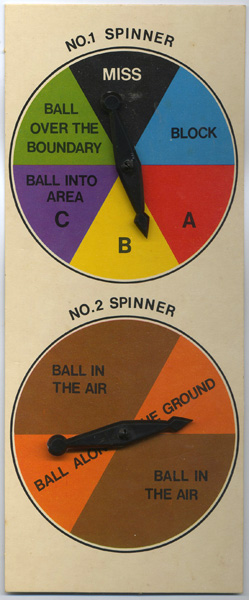
\includegraphics[height=2in]{img/family-cricket-spinner.jpg}
\end{minipage}
\vfill
\hfill {\tiny Image source: \url{http://replaycricket.com/2010/10/29/family-cricket/}}


\sld{Repeated i.i.d. Binary Trials}
%
\begin{itemize}
\item Suppose the outcome is binary and assigned to 0 or 1; e.g.,
\begin{subitemize}
\item 20\% chance of outcome 1: \emph{ball in play}
\item 80\% chance of outcome 0: \emph{ball \emph{not} in play}
\end{subitemize}
\item Consider different numbers of bowls delivered.
\item How will proportion of successes in sample differ?
\end{itemize}


\sld{Simulating i.i.d. Binary Trials}
%
\begin{itemize}
\item R Code: {\small \code{rbinom(10, N, 0.2) / N}}
\begin{subitemize}
\item {\bfseries 10 bowls} \hfill (10\% to 50\% success rate)
\\[4pt] 2 3 5 2 4 1 2 2 1 1
\vspace*{3pt}
%
\item {\bfseries 100 bowls} \hfill (16\% to 26\% success rate)
\\[4pt] 26 18 23 17 21 16 21 15 21 26
\vspace*{3pt}
%
\item {\bfseries 1000 bowls} \hfill (18\% to 22\% success rate)
\\[4pt] 181 212 175 213 216 179 223 198 188 194
\vspace*{3pt}
%
\item {\bfseries 10,000 bowls} \hfill (19.3\% to 20.3\% success rate)
\\[4pt] 2029 1955 1981 1980 2001 2014 1931 1982 1989 2020
\end{subitemize}
\end{itemize}


\sld{Pop Quiz! Cancer Clusters}
%
\begin{itemize}
\item Why do lowest and highest cancer clusters look so similar?
\end{itemize}
\vspace*{1pt}
\begin{center}
\hfill
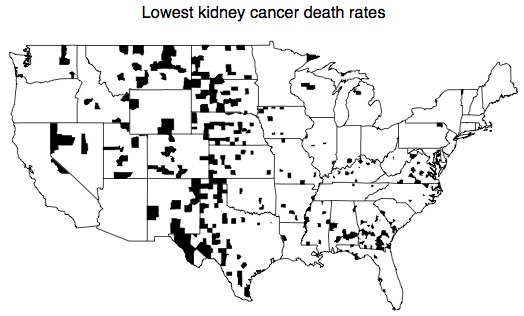
\includegraphics[width=0.45\textwidth]{img/low-cancer.jpg}
\hfill
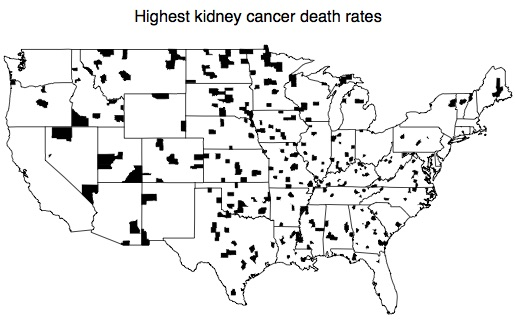
\includegraphics[width=0.45\textwidth]{img/high-cancer.jpg}
\hfill
\end{center}
\vfill
\hfill {\tiny Image from Gelman et al., {\slshape Bayesian Data Analysis, 3rd Edition} (2013)}


\sld{Pop Quiz Answer}
%
\begin{itemize}
\item Hint: mix earlier simulations of repeated i.i.d. trials with 20\% success and sort:
{\footnotesize
\begin{center}
\begin{tabular}{ccccc}
1/10 &  1/10 &  1/10 &  15/100 &  16/100
\\
17/100 &  175/1000 &  179/1000 &  18/100 &  181/1000
\\
188/1000 &  194/1000 &  198/1000 & 2/10 &  2/10
\\
2/10 &  2/10 & 21/100 &  21/100 &  21/100
\\
212/1000 &  213/1000 &   216/1000 &   223/1000 &  23/100
\\
26/100 &  26/100 &  3/10 &  4/10 &  5/10
\end{tabular}
\end{center}
}
\item More variation in observed rates with smaller sample sizes
\vfill
\item \emph{Answer}: High cancer and low cancer counties are small populations
\end{itemize}


\sld{Estimating Chance of Success}
%
\begin{itemize}
\item Estimate chance of success $\theta$ by proportion of successes:
\[
\theta^{*} = \frac{\text{successes}}{\text{attempts}}
\]
\item Simulation shows accuracy depends on the amount of data.
\item Statistics is about quantifying uncertainty.
\item Bayesian statistics is about using uncertainty in inference.
\end{itemize}

{\footnotesize Notation: $\theta^{*}$ denotes the
{\it maximum likelihood estimate} of $\theta$.}


\sld{Confidence via Simulation}
%
\begin{itemize}
\item Estimator uncertainty (\emph{not} Bayesian posterior)
{\small
\begin{Verbatim}
num_sims <- 10000
N <- 100;
theta <- 0.2;
hist(rbinom(num_sims, N, theta) / N,
     main=sprintf("%d simulations",N), xlab="theta*");
\end{Verbatim}
}
\vspace*{-12pt}
\begin{center}
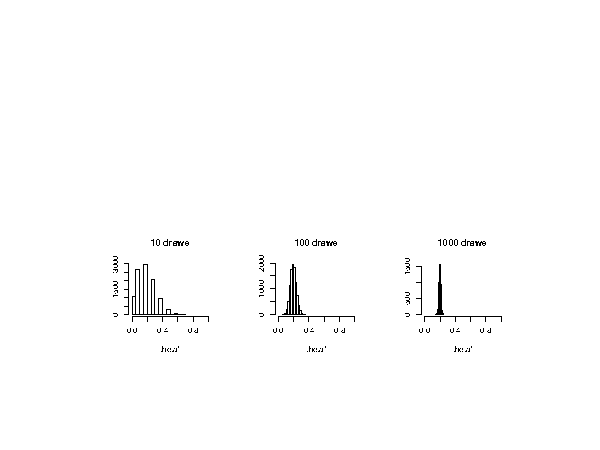
\includegraphics[width=0.8\textwidth]{img/hist-10-100-1000.pdf}
\end{center}
\end{itemize}


\sld{Example Interval Calculation}
%
\begin{itemize}
\item \emph{$P\%$ confidence interval:}  interval in which $P\%$ of the estimates are
expected to fall.
\item Simulation computes intervals to any accuracy.
\item Simulate, sort, and inspect the central empirical interval.
{\small
\begin{Verbatim}
> sims <- rbinom(10000, 1000, 0.2) / 1000
> sorted_sims <- sort(sims)
> sorted_sims[c(250, 9750)]
[1] 0.176 0.225
\end{Verbatim}
}
\item The 95\% confidence interval is thus $(0.176,0.225)$
\item i.e., if true $\theta = 0.2$, then 95\% of the samples of
  size 1000 used will produce estimates in $(0.176,0.225)$
\end{itemize}


\sld{Estimator Bias}
%
\begin{itemize}
\item {\bfseries Bias:} expected difference of estimate from true value
\item Continuing previous example
{\small
\begin{Verbatim}
> sims <- rbinom(10000, 1000, 0.2) / 1000
> mean(sims)
[1] 0.2002536
\end{Verbatim}
}
\item Value of 0.2 is estimate of expectation
\item Shows this estimator is \emph{unbiased}
\end{itemize}


\sld{Central Limit Theorem (picture)}
%
\vspace*{-3pt}
\begin{center}
\vspace*{-3pt}
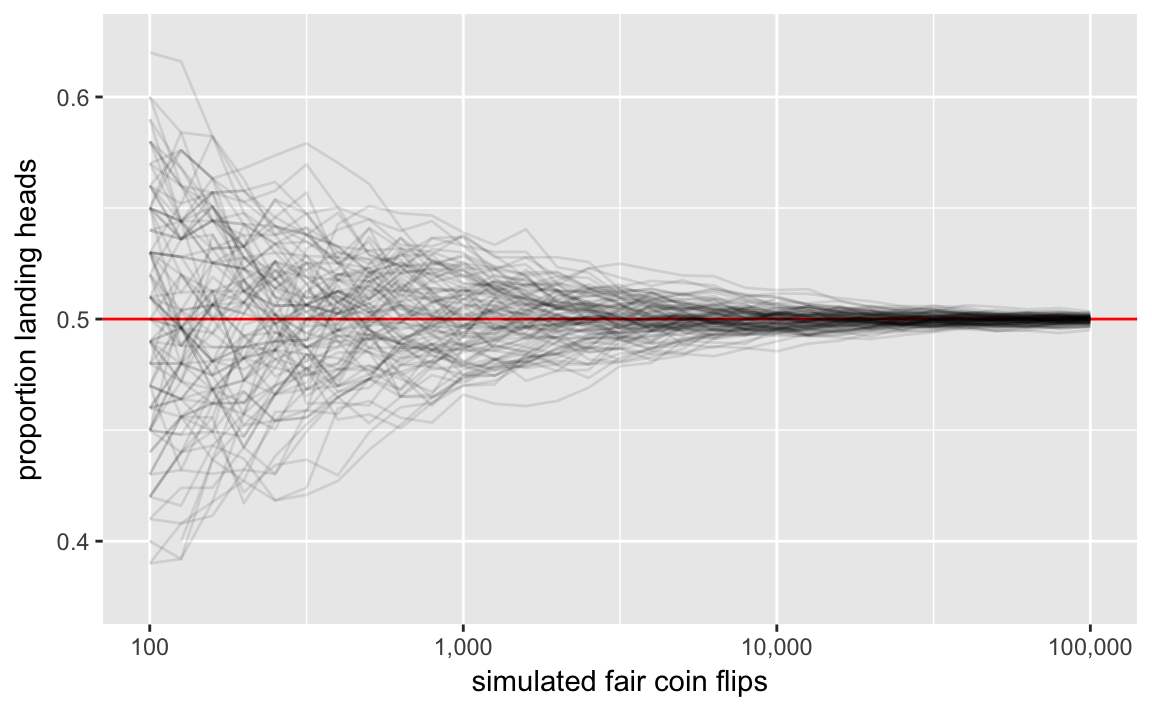
\includegraphics[width=0.8\textwidth]{img/coin-flip-clt.png}
\end{center}
\vspace*{-8pt}
\begin{subitemize}
\item proportion heads for 100 sequences of 100,000 flips
\vspace*{-2pt}
\item converges gradually to expected value of 0.5
\end{subitemize}


\sld{Central Limit Theorem (words)}
%
\begin{itemize}
\item \myemph{The} theorem of statistics
\vspace*{-4pt}
\begin{subsubitemize}
\item Cardano (1501--1576) conjectured convergence; (Jacob) Bernoulli
  (1713) proved convergence for binomials (law of large numbers); de Moivre
  (1733) conjectured the CLT; Laplace (1812) proved i.i.d.\ version;
  Lyapunov (1901) removed i.i.d.\ constraint
\end{subsubitemize}
\item Sample \myemph{mean} of $N$ i.i.d. variables with finite expectation
\begin{subitemize}
\item  \myemph{converges} to their expectation as $N \rightarrow \infty$
\vspace*{2pt}
\item \myemph{rate} of convergence is {\large ${\mathcal{O}}\!\left( \frac{1}{\sqrt{N}} \right)$}
\vspace*{2pt}
\item constant factor determined by standard deviation
\end{subitemize}
\vfill
\item Each decimal place of accuracy requires $100 \times$ more draws
\end{itemize}


\sld{Central Limit Theorem (math)}
%
\begin{itemize}
\item Simple i.i.d.\ version---can be established more generally
\item Given $N$ i.i.d.\ variables $\theta_1, \ldots, \theta_N$ with
\begin{subitemize}
\item $\mathbb{E}[\theta_n] = \mu$
\item $\mathrm{sd}[\theta_n] = \sigma$
\end{subitemize}
the \myemph{central limit theorem} states
%
\[
\lim_{N \rightarrow \infty} \
\frac{\theta_1 + \cdots + \theta_N}{N}
\sim
\mathsf{Normal}\left( \mu, \frac{\sigma}{\sqrt{N}} \right)
\]
\end{itemize}



\mypart{}{Numerical Analysis}

\sld{Floating-Point Standard: IEEE 754}
%
\begin{itemize}
\item \myemph{Finite numbers} ($s$: sign; $c$: mantissa; $q$: exponent)
{\large
\[
x = (-1)^s \times c \times 2^q
\]
}
\begin{center}
\begin{tabular}{r|c|c|cc}
{\slshape size} & $s, c$ {\slshape bits} & $q$ {\slshape bits}
& {\slshape range} & {\slshape precision}
\\ \hline
{\slshape 32-bit} & 24 & 8
& $\pm 3.4 \times 10^{38}$ & 7.2 digits
\\[4pt]
{\slshape 64-bit} & 53 & 11
& $\pm 1.8 \times 10^{308}$ & 16 digits
\end{tabular}
\end{center}
\item Quiet and signaling \myemph{not-a-number} (NaN)
\item Positive and negative \myemph{infinity} ($+\infty, -\infty$)
\item \myemph{Stan} uses 64-bit floating point
\end{itemize}


\sld{Catastrophic Cancellation}
%
\begin{itemize}
\item Subtraction risks \myemph{catastrophic cancellation}
\item Consider $0.99802 - 0.99801 = 0.00001$
\begin{subitemize}
\item input has five digits of precision
\item output has single digit of precision
\end{subitemize}
\item E.g., problem for sample variance of sequence $x$
\[
\mbox{var}(x) = \frac{1}{N - 1} \, \sum_{n = 1}^N (x_n - \overline{x})^2
\]
if elements $x_n$ close to sample mean
\[
\overline{x} = \frac{1}{N} \, \sum_{n=1}^N x_n
\]
\end{itemize}

\sld{Welford's Algorithm}
\begin{itemize}
\item \myemph{Streaming computation} uses fixed memory
\begin{stancode}
N = 0;    mean = 0;    sum_sq_err = 0

handle(y):
    N += 1
    diff = y - mean
    mean = mean + diff / N
    diff2 = y - mean
    sum_sq_err += diff * diff2

mean():  return mean

var():  return sum_sq_err / (N - 1)
\end{stancode}
\item Two stage difference is \myemph{less prone to cancellation}
\end{itemize}


\sld{Gaps Between Numbers}
%
\begin{itemize}
\item Smallest number greater than zero
\begin{subitemize}
\item single precision:  $1.4 \times 10^{-45}$
\item double precision: $4.9 \times 10^{-324}$
\end{subitemize}
\item Largest number less than one
\begin{subitemize}
\item single precision: $1 - 10^{-7.2}$
\item double precision: $1 - 10^{-16}$
\end{subitemize}
\item Gap size \myemph{depends on scale}
\end{itemize}


\sld{Lack of Transitivity}
%
\begin{itemize}
\item For real numbers $x, y, z \in \mathbb{R}$,
\[
x + (y + z) \ = \ (x + y) + z
\]
\item This can fail for floating point due to rounding
\begin{subitemize}
\item \code{(1 + 6e-17) + 6e-17 == 1}
\item \code{1 + (6e-17 + 6e-17) != 1}
\end{subitemize}
\item For square matrices $L \, L^{\top}$ is symmetric
\item This won't hold for efficient matrix multiplications
\begin{subitemize}
\item \code{(L * L')[1, 2] != (L * L')[2, 1]}
\end{subitemize}
\end{itemize}


\sld{Rounding and Equality}
%
\begin{itemize}
\item Dangerous to compare floating point numbers
\begin{subitemize}
\item they may have lost precision during calculation
\end{subitemize}
\item Rounding
\begin{subitemize}
\item default: round toward nearest
\item round toward zero, round to plus or minus infinity
\end{subitemize}
\end{itemize}


\sld{Overflow and Rounding}
%
\begin{itemize}
\item Because there is a max size, operations can overflow
\begin{subitemize}
\item e.g., \code{exp(1000)}, \code{1e200 * 1e200}, ...
\end{subitemize}
\item Because there are gaps, operations can round to zero
\begin{subitemize}
\item e.g., \code{exp(-1000)}, \code{1e-200 * 1e-200}, ...
\item e.g., evaluating $\prod_{n=1}^N p(y_n | \theta)$ underflows
for $N = 2000$ if $p(y_n | \theta) < 0.1$.
\end{subitemize}
\end{itemize}


\sld{Example: \code{log1p} and CCDFs}
%
\begin{itemize}
\item \code{log1p(x)} is for evaluating $\log$ near one
\begin{subitemize}
\item when \code{x} is near zero, \code{1 + x} catastrophically rounds
  to 1
\item this forces \code{log(1 + x)} to round to 0
\item \code{log1p(x)} avoids \code{1 + x} operation
\item \code{log1p(x)} uses Taylor series expansion of $\log(1 + x)$
\end{subitemize}
\item Complementary CDFs evaluate CDFs with values near one
\begin{subitemize}
\item $X$ is some random variable, e.g., $X \sim \mathsf{Normal}(0, 1)$
\item CDF: $F_X(x) = \mbox{Pr}[X \leq x]$
\item CCDF: $F^{\complement}_X(x) = 1 - \mbox{Pr}[X \leq x]$
\item converts range around one to range around zero
\end{subitemize}
\end{itemize}


\sld{Example: \code{log} and \code{log\_sum\_exp}}
%
\begin{itemize}
\item \myemph{Multiplication on the log scale}: \code{log}
\begin{subitemize}
\item $\log (a \times b) = \log a + \log b$
\item log converts multiplication to addition
\item $\log \prod_n x_n = \sum_n \log x_n$
\item avoids underflow and overflow even if $x_n \ll 1$ or $x_n \gg 1$
\item useful absolutely everywhere (e.g., log likelihoods)
\end{subitemize}
\item \myemph{Addition on the log scale}: \code{log\_sum\_exp}
\begin{subitemize}
\item $\log (a + b) = \log(\exp(\log a) + \exp(\log b))$
\item log converts addition to log sum of exponentials
\item avoids underflow and overflow, preserves precision
\item useful for mixtures (e.g., HMMs, zero-inflated Poisson)
\end{subitemize}
\end{itemize}


\sld{Example: \code{log\_sum\_exp}}
%
\begin{itemize}
\item Without loss of generality, assume $a > b$ (otherwise swap)
\vspace*{-8pt}
\begin{eqnarray*}
\mathrm{log\_sum\_exp}(a, b) & = & \log(\exp(a) + \exp(b))
\\[2pt]
& = & a + \log(\exp(a - a) + \exp(b - a))
\\[2pt]
& = & a + \log(1 + \exp(b - a))
\\[2pt]
& = & a + \mathrm{log1p(\exp(b - a))}
\end{eqnarray*}
\vspace*{-8pt}
\begin{subitemize}
\item \myemph{increase precision}: \ pull $a$ out of $\log()$ and
  $\exp()$
\item \myemph{increase precision}: \ use \code{log1p}
\item \myemph{prevents overflow}: \ can't overflow because $b - a \leq 0$
\end{subitemize}
\item Generalize to more than two inputs: subtract max
\end{itemize}





\mypart{}{Monte Carlo \\[8pt]\spc Integration}

\sld{Monte Carlo Calculation of $\pi$}

\noindent
\begin{minipage}[t]{0.65\textwidth}
\begin{itemize}
\item Computing $\pi = 3.14\ldots$ via simulation is \emph{the} textbook application
of Monte Carlo methods.
\vfill
\item Generate points uniformly at random within the square
\item Calculate proportion within circle ($x^2 + y^2 \leq 1$) and multiply by square's area (4) to produce the area of the circle.
\item This area is $\pi$ (radius is 1, so area is $\pi r^2 = \pi$)
\end{itemize}
\end{minipage}
%
\hfill
\begin{minipage}[t]{0.2\textwidth}
\vspace*{12pt}
\hfill 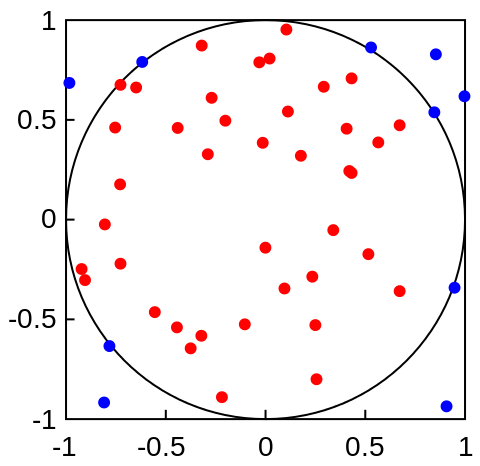
\includegraphics[height=\textwidth]{img/mc-integration-wikipedia.png}
\\[4pt]
{\tiny plot by Mysid Yoderj,\\ courtesy of Wikipedia.}
\end{minipage}
\vfill


\sld{Monte Carlo Calculation of $\pi$ {\normalsize (cont.)}}
%
\begin{subitemize}
\item R code to calculate $\pi$ with Monte Carlo simulation:
\\[-8pt]
{\small
\begin{Verbatim}
> x <- runif(1e6,-1,1)
> y <- runif(1e6,-1,1)

> prop_in_circle <- sum(x^2 + y^2 <= 1) / 1e6

> 4 * prop_in_circle
[1] 3.144032
\end{Verbatim}
}
\end{subitemize}


\sld{$\pi$ as an Expectation}
%
\begin{itemize}
\item If probability is uniform over the sample space,
\\[2pt] \ \ then an event's
  probability is its area (volume in general)
\item Suppose $X, Y \sim \mathsf{Uniform}(-1, 1)$
\item Then $\mathrm{Pr}[X^2 + Y^2 \leq 1] \ = \ \pi / 4$.
\item To calculate using Monte Carlo draws $(x^{(m)}, y^{(m)})$,
{\small
\begin{eqnarray*}
\mathrm{Pr}[X^2 + Y^2 \leq 1]
& = & \mathbb{\normalsize E}\!\left[ \, \mathrm{\normalsize I}\!\left[ X^2 + Y^2 < 1 \right]
      \, \right]
\\[8pt]
& = & \int_{-1}^1 \int_{-1}^1 \
       \mathrm{\normalsize I}\!\left[ x^2 + y^2 < 1 \right] \ p_X(x) \ p_Y(y) \ \mathrm{d}x \, \mathrm{d}y
\\[8pt]
& \approx
& \frac{1}{M}
\ \mathrm{\Large I}\!\left[ \left( x^{(m)} \right)^2 + \left( y^{(m)} \right)^2
                   < 1 \right]
\end{eqnarray*}
}
\end{itemize}

\sld{Calculating $\pi$ with Stan}
%
\begin{itemize}
\item Complete Stan program to compute $\mathrm{Pr}[X^2 + Y^2 \leq 1]$:
\begin{stancode}
generated quantities {
  real x = uniform_rng(-1, 1);
  real y = uniform_rng(-1, 1);
  real pi_div_4 = hypot(x, y) <= 1;
}
\end{stancode}
\item \myemph{Simulates} $X$ and $Y$
\item \myemph{Codes indicator function} implicitly with comparison
\begin{subitemize}
\item uses Stan's built-in hypotenuse function
\item \Verb|hypot(a, b) = sqrt(a^2 + b^2)|
\end{subitemize}
\end{itemize}

\sld{Fitting Stan model for $\pi$ in R}
\begin{itemize}
\item \code{Fixed\_param} algorithm for no parameters
\begin{stancode}
> fit <- stan("pi.stan", algorithm="Fixed_param",
              iter=100000)
\end{stancode}
\item Print only what's needed (print output elided manually)
\begin{stancode}
> print(fit, digits=3, probs=c(), pars=c("pi_div_4"))

          mean se_mean
pi_div_4 0.786   0.001
\end{stancode}
\item Estimate accurate to \myemph{within estimated tolerances}
\begin{subitemize}
\item $4 \times 0.786 = 3.144$
\item predicted accuracy is 0.004 (four times standard error)
\end{subitemize}
\end{itemize}


\sld{Accuracy of Monte Carlo}
%
\begin{itemize}
\item Monte Carlo Integration computes the exact posterior to within any $\epsilon$
(\emph{not} like variational Bayes which yields an approximation of the posterior)
\item Monte Carlo draws are i.i.d. by definition
\item Central limit theorem: expected error decreases at rate of
{\Large
\[
\frac{1}{\sqrt{N}}
\]
}
\item 3 decimal places of accuracy with
sample size 1e6
\item Need $100 \times$ larger sample for each digit of accuracy
\end{itemize}


\sld{General Monte Carlo Integration}
%
\begin{minipage}[t]{0.69\textwidth}
\vspace*{-0.1in}
\small
\begin{itemize}
\item MC can calculate arbitrary definite integrals,
\[
\int_a^b f(x) \, dx
\]
\item Let $d$ upper bound $f(x)$ in $(a,b)$;  tightness determines
computational efficiency
\item Then generate random points uniformly in the rectangle bounded by $(a,b)$ and $(0,d)$
\item Multiply proportion of draws $(x,y)$ where $y < f(x)$ by area of rectangle, $d \times (b-a)$.
\item Can be generalized to multiple dimensions in obvious way
\end{itemize}
\end{minipage}
\begin{minipage}[t]{0.29\textwidth}
\mbox{ } \\
\mbox{ } \ \ \ \
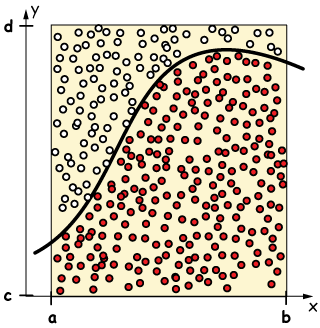
\includegraphics[height=0.9in]{img/monte-carlo-integration.png}
\end{minipage}
\vfill
\hfill
{\tiny Image courtesy of Jeff Cruzan, \url{http://www.drcruzan.com/NumericalIntegration.html}}


\sld{Expectations of Function of R.V.}
%
\begin{itemize}
\item Suppose $f(\theta)$ is a function of random variable vector
  $\theta$
\item Suppose the density of $\theta$ is $p(\theta)$
\begin{subitemize}
\item {\slshape Warning}: $\theta$ overloaded as random and bound variable
\end{subitemize}
\item Then $f(\theta)$ is also random variable, with expectation
  \[
  \mathbb{E}[f(\theta)] = \int_{\Theta} f(\theta) \ p(\theta) \ d\theta.
  \]
\begin{subitemize}
\item
where $\Theta$ is support of $p(\theta)$ (i.e., $\Theta =
\setcomp{\theta \, | \, p(\theta) > 0}$
\end{subitemize}
\end{itemize}


\sld{QoI as Expectations}
%
\begin{itemize}
\item Most Bayesian quantities of interest (QoI) are expectations
  over the posterior $p(\theta \, | \, y)$ of functions $f(\theta)$
\item \myemph{Bayesian parameter estimation}: $\hat{\theta}$
\begin{subitemize}
\item $f(\theta) = \theta$
\item $\hat{\theta} = \mathbb{E}[\theta | y]$ minimizes expected
  square error
\end{subitemize}
\item \myemph{Bayesian parameter (co)variance estimation}:
  $\mathrm{var}[\theta \, | \, y]$
\begin{subitemize}
\item $f(\theta) = (\theta - \hat{\theta})^2$
\end{subitemize}
\item \myemph{Bayesian event probability}:  $\mbox{Pr}[A \, | \, y]$
\begin{subitemize}
  \item $f(\theta) = \mathrm{I}(\theta \in A)$
\end{subitemize}
\end{itemize}


\sld{Expectations via Monte Carlo}
%
\begin{itemize}
\item Generate draws $\theta^{(1)}, \theta^{(2)}, \ldots,
  \theta^{(M)}$ drawn from $p(\theta)$
\item Monte Carlo Estimator \myemph{plugs in average} for expectation:
  \[
  \mathbb{E}[f(\theta)|y] \approx \frac{1}{M} \sum_{m=1}^M f(\theta^{(m)})
  \]
\item Can be made \myemph{as accurate as desired}, because
\[
\mathbb{E}[f(\theta)]
=
\lim_{M \rightarrow \infty} \
\frac{1}{M} \sum_{m=1}^M f(\theta^{(m)})
\]
\vfill
\item {\slshape Reminder}:  By CLT, error goes down as
$1 \, / \, \sqrt{M}$
\end{itemize}


\mypart{}{The Curse of\\[8pt]{\spc}Dimensionality}


\sld{The Curse}
%
\begin{itemize}
\item Intuitions formed in low dimensions break down \myemph{do not
    generalize}
\item In high dimensions, \myemph{everything is far away}
\begin{subitemize}
\item random draws are far away from each other
\item random draws are far away from the mode or meaan
\end{subitemize}
\item Sampling algorithms that work in low dimensions often \myemph{fail
  in high dimensions}
\end{itemize}

\sld{Volume of Ball in Cube}
%
% need newline here

\noindent
\begin{minipage}[t]{0.6\textwidth}
\vspace*{-1.7in}
\begin{subitemize}
\item Assume $x, y, z \sim \mathsf{Uniform}(-1, 1)$,
\item $\mbox{Pr}[(x,y,z) \in \mbox{unit ball}]$ \hfill
\\ is unit ball's fraction of volume.
\item Analytic solution:
\\[4pt]\hspace*{-1em}
$\int_{-1}^1 \int_{-1}^1 \int_{-1}^1 \,
\mathrm{I}[ x^2 + y^2 + z^2 \leq 1 ] \,
\mathrm{d} x \, \mathrm{d} y \, \mathrm{d} z$

\item Monte Carlo solution:
\begin{subsubitemize}
\item simulate multiple $(x, y, z)$ uniformly in cube
\item count proportion in ball, i.e., \\[4pt]
$x^2 + y^2 + z^2 \leq 1$
\end{subsubitemize}
\end{subitemize}
\end{minipage}
\hfill
\begin{minipage}[t]{0.4\textwidth}
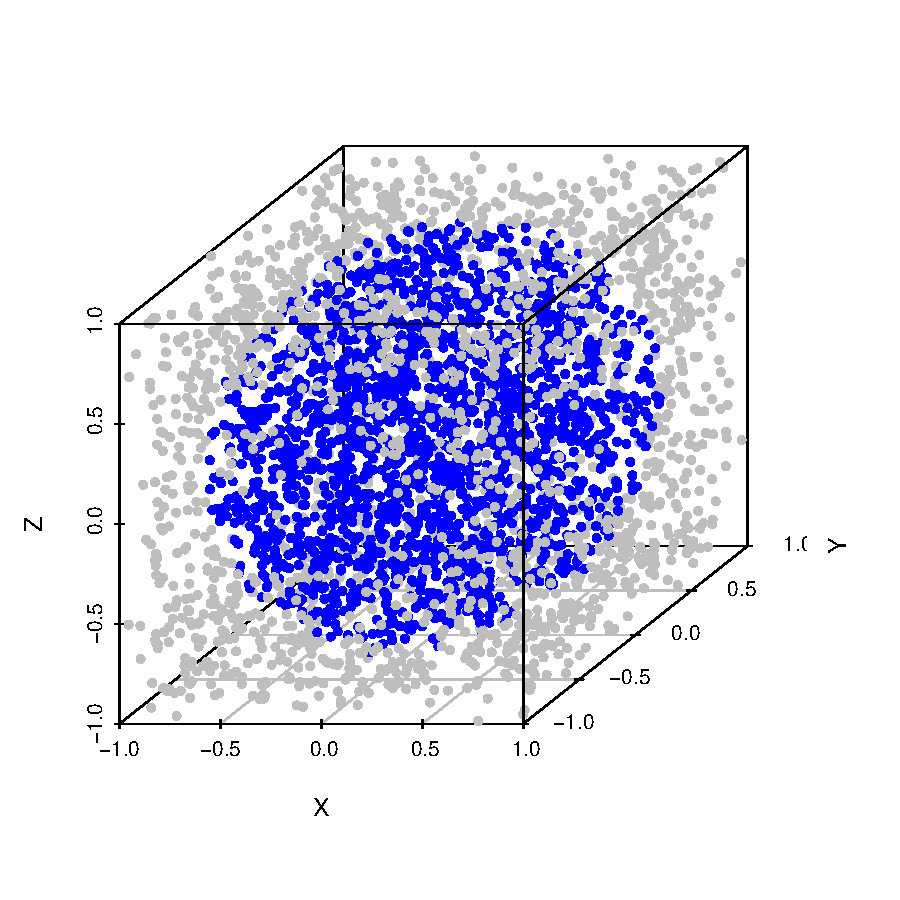
\includegraphics[width=1.2\textwidth]{img/ball-in-cube.pdf}
\\[-12pt]
{\footnotesize\slshape \hspace*{0.5in}4000 simulations;
\\\hspace*{0.5in}blue inside unit ball.}
\end{minipage}

% Key R for that plot:
% X = runif(4000, -1, 1)
% pcolor = rep("gray", 4000)
% pcolor[X * X + Y * Y + Z * Z <= 1] = "blue"
% scatterplot3d(X, Y, Z, pch=19, color=pcolor)

\sld{Ball in Cube in Stan}
%
\begin{stancode}
generated quantities {
  int<lower = 0, upper = 1> in_ball;
  {
    real x = uniform_rng(-1, 1);
    real y = uniform_rng(-1, 1);
    real z = uniform_rng(-1, 1);
    in_ball = (x^2 + y^2 + z^2 <= 1);
  }
}
\end{stancode}
\begin{subitemize}
\item \code{in\_ball} is value of indicator (implicit in \code{<=}).
\item Posterior mean of \code{in\_ball} is fraction draws in ball.
\item Posterior mean estimates $\mbox{Pr}[x^2 + y^2 + z^2 \leq 1]$.
\end{subitemize}

\sld{Ball in Cube in Stan from RStan}
%
\begin{itemize}
\item Use the \code{Fixed\_param} algorithm:

\begin{stancode}
> fit <- stan("ball-in-cube.stan",
               algorithm="Fixed_param",
              iter=10000)

> print(fit, probs=c(), digits=3)

         mean se_mean    sd n_eff Rhat
in_ball 0.528   0.004 0.499 19400    1
\end{stancode}
\item Thus $\mbox{Pr}[X^2 + Y^2 + Z^2 \leq 1] \approx 0.53$
\item with standard error of 0.004, yielding a 95\% interval of $\pm
  0.008$, i.e., roughly (0.52, 0.54)
\end{itemize}

\sld{Hyperballs in Hypercubes}
%
\begin{itemize}
\item \myemph{sample uniformly} from container (square, cube, ...)
\item 2 dimensions $(x, y)$: compute $\mbox{Pr}[X^2 + Y^2 \leq 1]$
  \begin{subitemize}
  \item unit \myemph{disc} inscribed in square
  \item calculate $\pi$ given known area of circle ($2 \pi$)
  \end{subitemize}
\item 3 dimensions $(x, y, z)$: compute $\mbox{Pr}[X^2 + Y^2 + Z^2 \leq 1]$
  \begin{subitemize}
  \item unit \myemph{ball} inscribed in cube
  \end{subitemize}
\item $N$-dimensions $(x_1, \ldots, x_N)$: compute $\mbox{Pr}[X_1^2 +
  \cdots X_N^2 \leq 1]$
  \begin{subitemize}
  \item unit \myemph{hyperball} inscribed in hypercube
  \end{subitemize}
\item Code event probability as \myemph{expectation of indicator}
\end{itemize}

\sld{Hyperballs in Hypercubes in Stan}
\vspace*{-8pt}
\begin{stancode}
generated quantities {
  int<lower=0, upper=1> in_ball[10];
  {
    real len = 0;
    for (n in 1:10) {
      len = len + uniform_rng(-1, 1)^2;
      in_ball[n] = (len <= 1);
    }
  }
}
\end{stancode}
%
\begin{subitemize}
\item draw $x_1, \ldots, x_N$ is implicit in \code{uniform\_rng}
\item \code{in\_ball[n]} is 1 iff $x_1^2 + \cdots + x_n^2 \leq 1$; \
  coded as indicator \Verb|(len <= 1)|
\item sum of squares accumulation reduces quadratic time to linear
\end{subitemize}

\sld{Hyperballs in Hypercubes in RStan}
\begin{stancode}
> fit <- stan("hyperballs.stan", algorithm="Fixed_param",
              iter=1e4)

> print(fit, probs=c())

            mean se_mean   sd n_eff Rhat
in_ball[1]  1.00       0 0.00 20000  NaN
in_ball[2]  0.78       0 0.41 20000    1
in_ball[3]  0.52       0 0.50 20000    1
in_ball[4]  0.31       0 0.46 20000    1
in_ball[5]  0.17       0 0.38 20000    1
in_ball[6]  0.08       0 0.27 20000    1
in_ball[7]  0.04       0 0.19 18460    1
in_ball[8]  0.02       0 0.12 19370    1
in_ball[9]  0.01       0 0.08 20000    1
in_ball[10] 0.00       0 0.05 20000    1
\end{stancode}

\sld{Proportion Volume in Hyperball}
%
\\
\spc
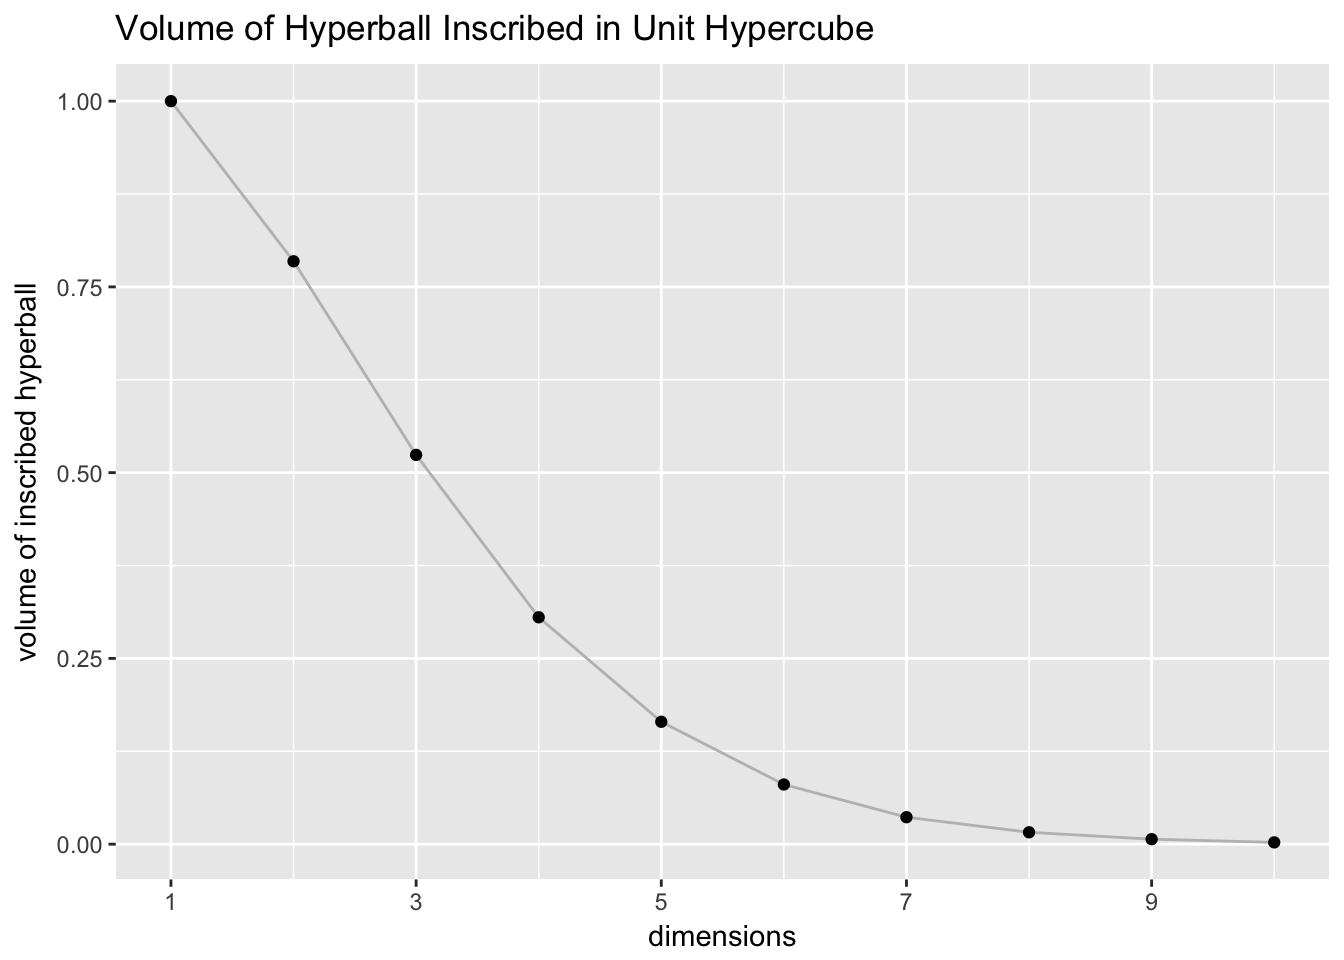
\includegraphics[width=0.825\textwidth]{img/volume-hyperball.png}




\mypart{}{Typical Sets}


\sld{Typical Set Example (1)}
%
\begin{itemize}
\item Consider a game of chance with an 80\% chance of winning
\item Play the game 100 times independently
\vfill
\item What is most likely outcome?
\end{itemize}

\sld{Typical Set Example (2)}
%
\begin{itemize}
\item For each trial, there is a 80\% chance of success
\item For each trial, most likely outcome is success
\item Overall, the single \myemph{most likely outcome} is all successes
\vfill
\item What's the \myemph{most likely number of successes}?
\end{itemize}

\sld{Typical Set Example (3)}
%
\begin{itemize}
\item Let $y_n \sim \mathsf{Bernoulli}(0.9)$ for $n \in 1:100$ be the trials
\item Expected number of successes
\begin{eqnarray*}
\textstyle
\mbox{\large $\mathbb{E}$}\!\left[ \sum_{n=1}^{100} y_n \right]
& = & \textstyle \sum_{n = 1}^{100} \mathbb{\large E}\!\left[ y_n \right]
\\[4pt]
& = & \textstyle \sum_{n=1}^{100} 0.8
\\[4pt]
& = & 0.8 \times 100
\\[2pt]
& = & 80
\end{eqnarray*}
\item \myemph{most likely outcome} (all successes) \myemph{is an
    outlier}!
\[
\mbox{Pr}[100 \ \mbox{successes}] = 0.8^{100} < 10^{-10}
\]
\end{itemize}

\sld{Typical Set Example (4)}
%
\begin{itemize}
\item Maximum likelihood (most likely) outcome is \myemph{atypical}
\item Expectations involve count times probability
\item 100 success sequences:
$\binom{100}{100} \ = \ \frac{100!}{100! \ \times \ 1!} \ = \ 1$
\item 80 success sequences:
$\binom{100}{80} \ = \ \frac{100!}{80! \ \times \ 20!} \ > \ 10^{20}$
\item Thus chance of 80 success is much higher than 100
\begin{eqnarray*}
\mathsf{Binomial}(80 \mid 100, 0.8)
& = &
  \textstyle \binom{100}{20} \times 0.8^{80} \times 0.2^{20}
\\[4pt]
& \gg &
\textstyle \binom{100}{1} \times 0.8^{100}
\\[4pt]
& = &
\mathsf{Binomial}(100 \mid 100, 0.8)
\end{eqnarray*}
\end{itemize}


\sld{Typical Set}
%
\begin{itemize}
\item Goal is to \myemph{evaluate posterior expectations using draws}
\begin{eqnarray*}
\mathbb{E}\left[ f(\theta) \mid y \right]
& = & \int_{\Theta} \, f(\theta) \, p(\theta | y) \, \mathrm{d}\theta
\\[4pt]
& \approx & \frac{1}{M} \, \sum_{m=1}^M f(\theta^{(m)})
\end{eqnarray*}
\item A \myemph{typical set} $A_{\epsilon}$ (at some level) is the set
\begin{subitemize}
\item of values with typical log density (near distribution entropy)
\item containing $1 - \epsilon$ of the probability mass
\end{subitemize}
\item A typical set $A_{\epsilon}$ \myemph{suffices for integration}
\[
\int_{\Theta} \, f(\theta) \, p(\theta | y) \, \mathrm{d}\theta
\ = \
\int_{A_{\epsilon}} \, f(\theta) \, p(\theta | y) \, \mathrm{d}\theta
\]
\end{itemize}


\mypart{}{Concentration\\[8pt]\spc of Measure}


\sld{Concentration of Measure}
%
\begin{itemize}
\item We care about probability \myemph{mass}, not \myemph{density}
\item Events with non-zero probability have probability mass, e.g.,
  $\mbox{Pr}[\theta_0 > \theta_1 \mid y]$
\item Mass arises from integrating over density
\item As data size increases, posterior concentrates around true value
\end{itemize}

\sld{E.g., Binomial Concentration}
%
\begin{itemize}
\item $y \sim \mathsf{Binomial}(N, \theta)$
\[
\mathsf{Binomial}(y \mid N, \theta)
= \binom{N}{y} \, \theta^y \, (1 - \theta)^{N - y}
\]
\item As $N \rightarrow \infty$, posterior average $y / N$
  concentrates around $\theta$
\item Concentration governed by central limit theorem
\end{itemize}

\sld{Binomial Concentration, $N = 25$}
%
\\[-12pt]
\begin{center}
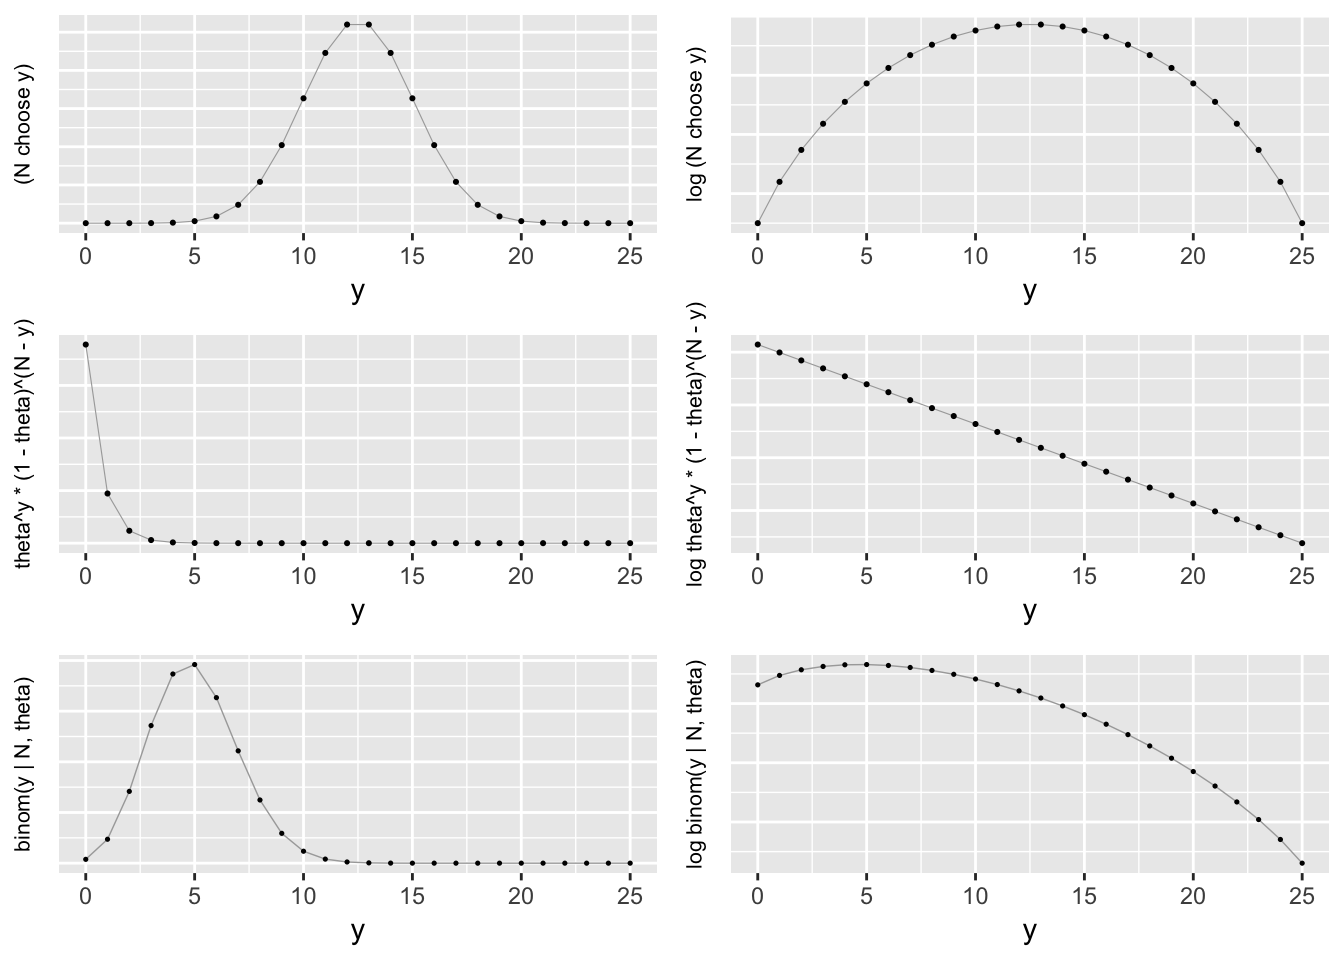
\includegraphics[width=0.8\textwidth]{img/binomial-concentration-25.png}
\end{center}

\sld{Binomial Concentration, $N = 100$}
%
\\[-12pt]
\begin{center}
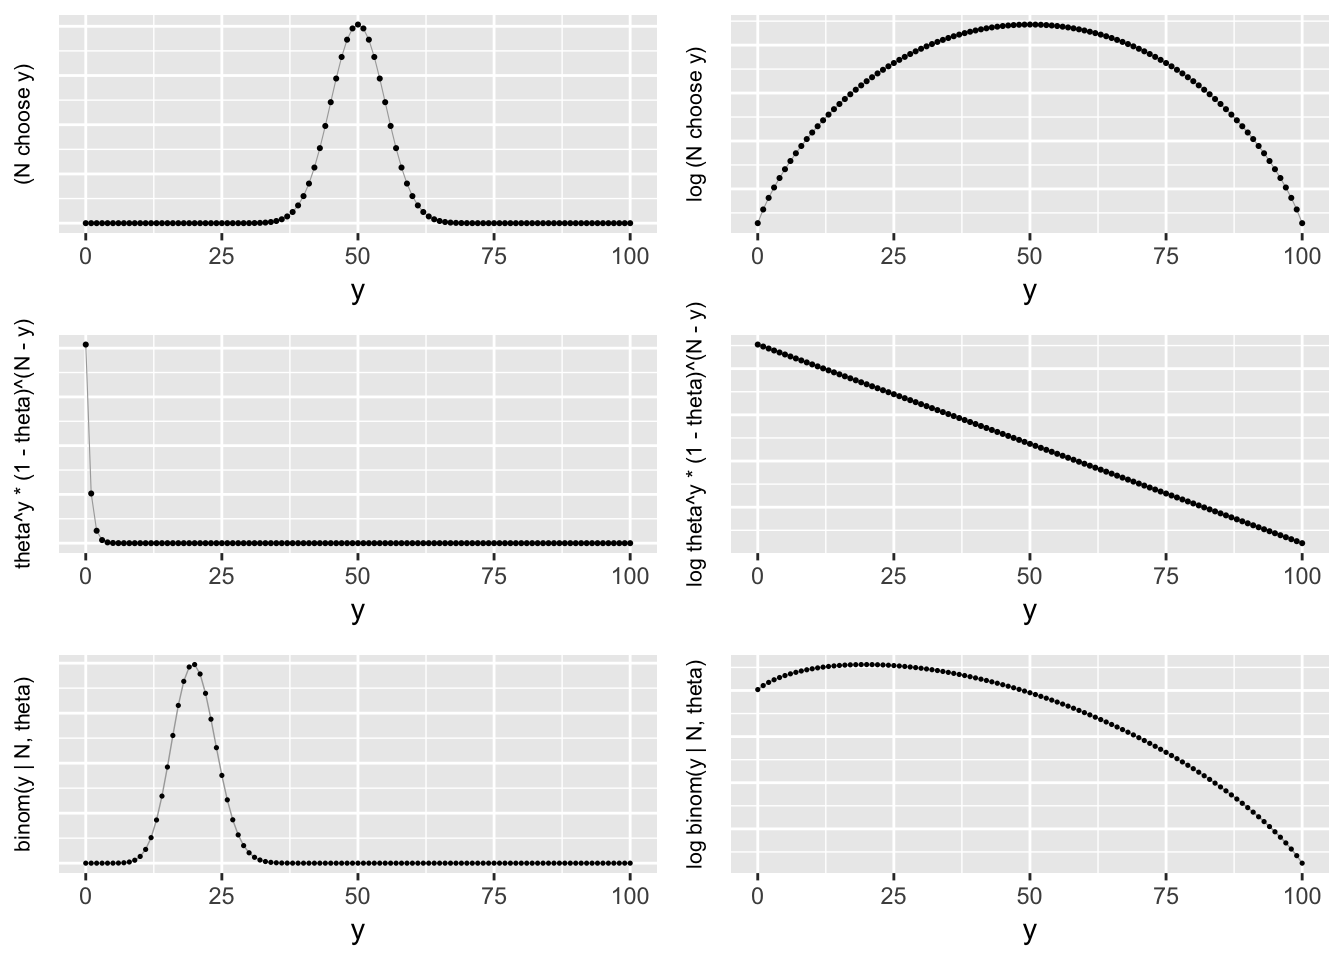
\includegraphics[width=0.8\textwidth]{img/binomial-concentration-100.png}
\end{center}

\sld{Binomial Concentration, $N = 400$}
%
\\[-12pt]
\begin{center}
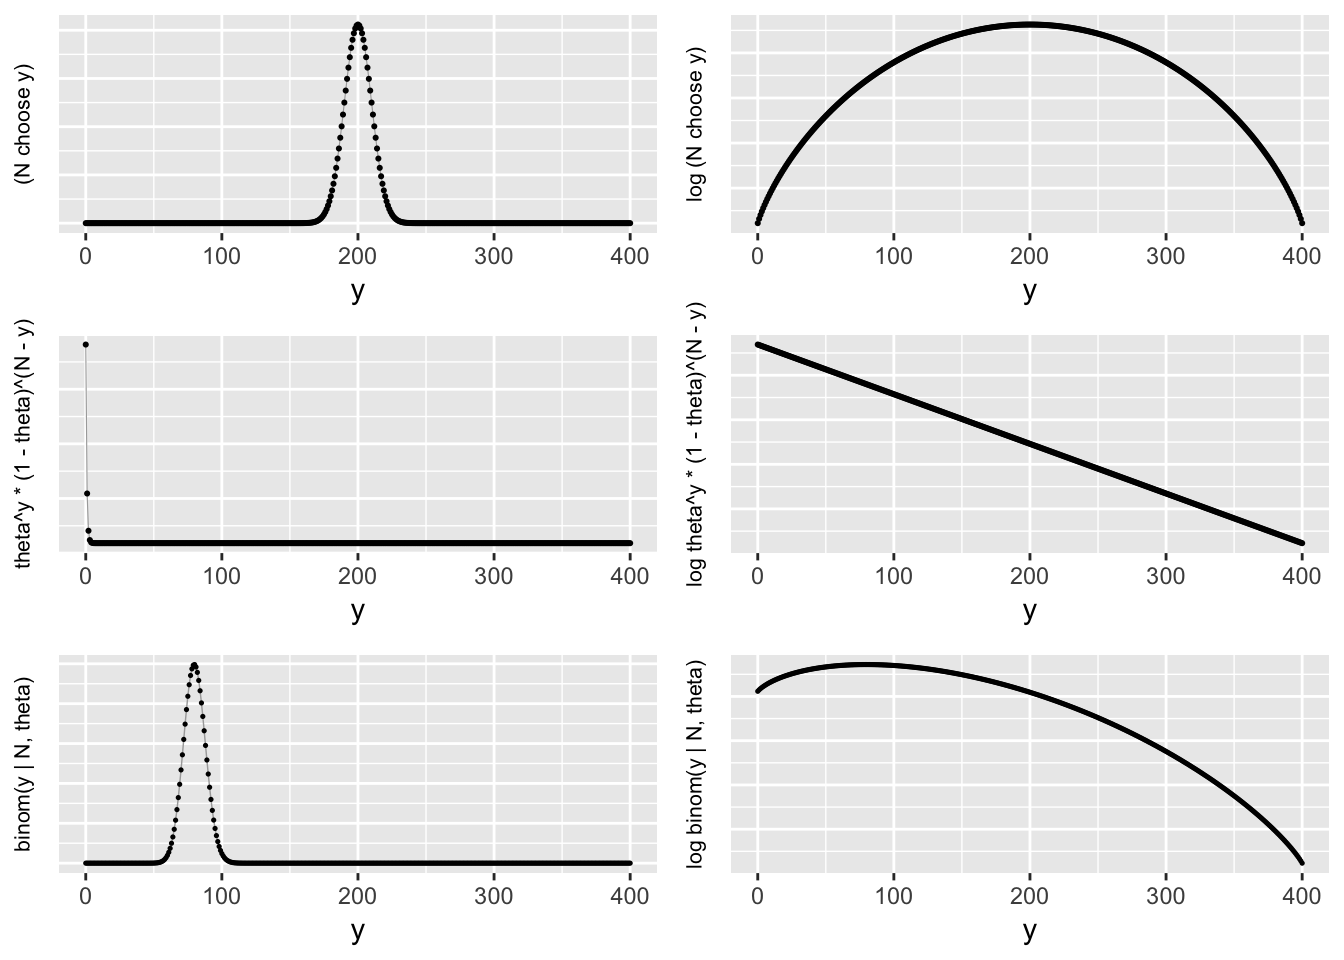
\includegraphics[width=0.8\textwidth]{img/binomial-concentration-400.png}
\end{center}


\sld{Continuous Hypervolumes}
%
\begin{itemize}
\item Generalize discrete to continuous
\begin{subitemize}
\item discrete: combinations times probability mass
\item continuous: volume times probabilty density
\end{subitemize}
\item Volume of ball at given radius ($r$) grows exponentially with
  dimension ($d$):
{\large
\[
\mbox{volume} \propto r^d
\]
}
\vspace*{-18pt}
\begin{subitemize}
\item line has length ${} \propto r$
\item disc has area ${} \propto r^2$
\item ball has volume ${} \propto r^3$
\item 4-dimensional hyperball has volume ${} \propto r^4$
\end{subitemize}
\end{itemize}




\mypart{}{Markov Chain \\[8pt]\spc{}Monte Carlo}


\sld{Markov Chain Monte Carlo}
%
\begin{itemize}
\item Standard Monte Carlo draws i.i.d. samples
\[
\theta^{(1)}, \ldots, \theta^{(M)}
\]
according to a probability function $p(\theta)$
\item Drawing i.i.d. samples typically impossible for
  complex densities like Bayesian posteriors $p(\theta|y)$
\item Instead, use Markov chain Monte Carlo (MCMC) to
  draw $\theta^{(1)}, \ldots, \theta^{(M)}$ from a Markov chain
  with appropriate stationary distribution $p(\theta | y)$.
\end{itemize}


\sld{Markov Chains}
%
\begin{itemize}
\item A Markov Chain is a sequence of random variables
\[
\theta^{(1)},
  \theta^{(2)}, \ldots, \theta^{(M)}
\]
such that $\theta^{(m)}$ only depends on $\theta^{(m-1)}$, i.e.,
\[
p(\theta^{(m)} | y, \theta^{(1)}, \ldots, \theta^{(m-1)})
\ = \
p(\theta^{(m)} | y, \theta^{(m-1)})
\]
\end{itemize}

\sld{Markov Chain Monte Carlo}
%
\begin{itemize}
\item Simulating independent draws from the posterior $p(\theta | y)$ usually intractable
\item Simulating a Markov chain $\theta^{(1)}, \ldots, \theta^{(M)}$
  with marginals equal to posterior, i.e.,
\[
p(\theta^{(m)} | y) = p(\theta | y)
\]
often is tractable
\item Replace indepedent draws with Markov chain of draws
\begin{subitemize}
\item Plug in just like ordinary (non-Markov chain) Monte Carlo
\item Adjust standard errors for correlation in Markov chain
\end{subitemize}
\end{itemize}


\mypart{}{MCMC Algorithms}


\sld{Random-Walk Metropolis}
%
\begin{itemize}
\item Draw random initial parameter vector $\theta^{(1)}$ (in
  support)
\item For $m \in \range{2}{M}$
\hspace*{-8pt}
\begin{subitemize}
\item Sample proposal from a (symmetric) jumping distribution, e.g.,
\[
\theta^*
\ \sim \
\distro{MultiNormal}(\theta^{(m-1)}, \ \sigma \mbox{\bfseries I})
\]
where {\bfseries I} is the identity matrix
\item
\vspace*{4pt}
Draw $u^{(m)} \sim \distro{Uniform}(0,1)$ and set
\[
\theta^{(m)}
\ = \
\begin{cases}
\theta^{*}
  & \text{if } u^{(m)} < {\displaystyle \frac{p(\theta^{*}|y)}{p(\theta^{(m)}|y)}}
\\[8pt]
\theta^{(m-1)}
  & \text{otherwise}
\end{cases}
\]
\end{subitemize}
\end{itemize}


\sld{Metropolis and Normalization}
%
\begin{itemize}
\item Metropolis only uses posterior in a ratio
\begin{eqnarray*}
\frac{p(\theta^{*} \, | \, y)}
     {p(\theta^{(m)} \, | \, y)}
& = &
\frac{p(y, \theta^*) \ / \ p(y)}
     {p(y, \theta^{(m)}) \ / \ p(y)}
\\[8pt]
& = &
\frac{p(y, \theta^*)}
     {p(y, \theta^{(m)})}
\\[8pt]
& = &
\frac{p(y \mid \theta^*) \, p(\theta^*)}
     {p(y \mid \theta^{(m)}) \, p(\theta^{(m)})}
\end{eqnarray*}
\item Drops $p(y)$ term with nasty integral
\item Baye's rule reduces to likelihood and prior
\end{itemize}


\sld{Metropolis-Hastings}
%
\begin{itemize}
\item Generalizes Metropolis to asymmetric proposals
\item Acceptance ratio is
\[
\frac{J(\theta^{(m)}|\theta^{*}) \ \times \ p(\theta^{*}|y)}
     {J(\theta^{*}|\theta^{(m-1)}) \ \times \ p(\theta^{(m)}|y)}
\]
where $J$ is the (potentially asymmetric) proposal density
\item i.e.,
{\small
\[
\frac{\mbox{density at } \theta^*
      \mbox{ and jump to } \theta^{(m-1)}}
     {\mbox{density at } \theta^{(m-1)}
      \mbox{ and jump to } \theta^{*}}
\]
}
\vspace*{3pt}
\item Like Metropolis, only requires ratios
%\item General form ensures equilibrium
%  by maintaining \emph{detailed balance}
%\item Can use volumes and measure rather than points and density
%\item Many algorithms involve a Metropolis-Hastings ``correction''
\end{itemize}


\sld{Detailed Balance \& Reversibility}
%
\begin{itemize}
\item Sufficient for a \emph{stationary distribution} on Markov chain
\[
p(\theta^{(m)}) = p(\theta) \ \mbox{ for all } m \gg 1
\]
\item Suppose $\pi(\theta^{(m+1)} | \theta^{(m)})$ is Markov transition density
\item Detailed balance is a reversibility equilibrium condition of
\begin{subitemize}
\item density at $\theta^{(m)}$ and jump density to $\theta^{(m+1)}$
\item density at $\theta^{(m+1)}$ and jump density back to
  $\theta^{(m)}$
\end{subitemize}
\[
p(\theta^{(m)}) \times \pi(\theta^{(m+1)} | \theta^{(m)})
\ = \
p(\theta^{(m+1)}) \times \pi(\theta^{(m)} | \theta^{(m+1)})
\]

\end{itemize}


\sld{Optimal Proposal Scale?}
%
\begin{subitemize}
\item Proposal scale $\sigma$ is a free; too low or high is inefficient
\begin{center}
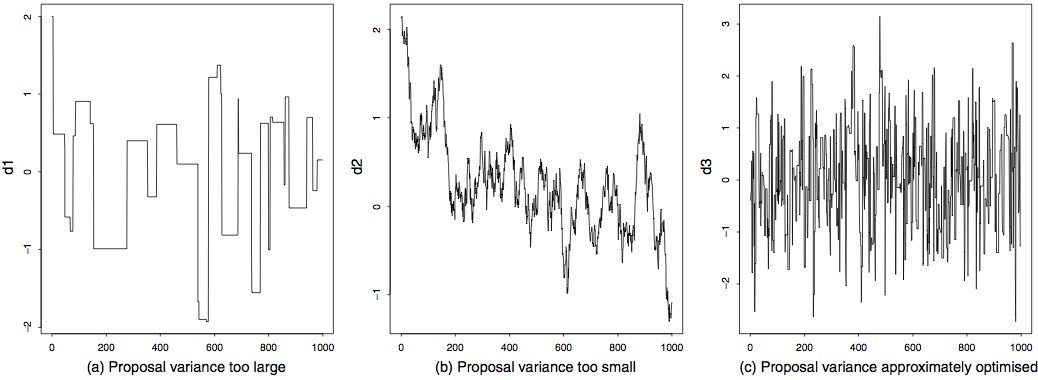
\includegraphics[width=0.9\textwidth]{img/roberts-rosenthal-traceplots.jpg}
\end{center}
\item \emph{Traceplots} show parameter value on $y$ axis, iterations on $x$
\item Empirical tuning problem; theoretical optima exist for some
  cases
\end{subitemize}
\vfill\hfill
{\tiny Roberts and Rosenthal (2001) Optimal Scaling for Various
  Metropolis-Hastings Algorithms. {\slshape Statistical Science}.}


\sld{Convergence and Stationarity}
%
\begin{itemize}
%\item Imagine releasing a hive of bees in a sealed house
%\begin{subitemize}
%\item they disperse, but eventually reach equilibrium where the same
%  number of bees leave a room as enter it (on average)
%\end{subitemize}
\item May take many iterations for chain to reach equilibrium
\item Different initializations should converge in distribution
\vspace*{3pt}
\begin{center}
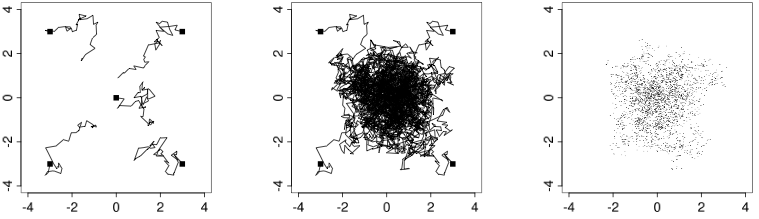
\includegraphics[width=0.8\textwidth]{img/bda-diffuse-converge.png}
\end{center}
\item Four chains with different starting points.  \emph{Left}) 50 iterations;  \emph{Center}) 1000 iterations;  \emph{Right}) Draws from second half of each chain
\end{itemize}


\sld{Potential Scale Reduction ($\hat{R}$)}
%
\begin{subitemize}
\item Gelman \& Rubin recommend $M$ chains of $N$ draws with
  \myemph{diffuse initializations}
\item Measure that each chain has same posterior mean and variance
\item If not, may be stuck in multiple modes or just not converged yet
\item Define statistic $\hat{R}$ of chains such that \myemph{at convergence},
$\hat{R} \rightarrow 1$
\begin{subsubitemize}
\item $\hat{R} >\!> 1$ implies non-convergence
\item $\hat{R} \approx 1$ \myemph{does not guarantee convergence}
\item Only measures marginals
\end{subsubitemize}
\end{subitemize}


\sld{Split $\hat{R}$}
\begin{itemize}
\item Vanilla $\hat{R}$ may not diagnose non-stationarity
\begin{subitemize}
\item e.g., a sequence of chains with an increasing parameter
\end{subitemize}
\item \myemph{Split $\hat{R}$}: \ Stan splits each chain into first and
  second half
\begin{subitemize}
\item start with $M$ Markov chains of $N$ draws each
\item split each in half to creates $2M$ chains of $N/2$ draws
\item then apply $\hat{R}$ to the $2M$ chains
\end{subitemize}
\end{itemize}


\sld{Calculating $\hat{R}$ Statistic}
%
\begin{subitemize}
\item \myemph{Between-sample variance} estimate
\[\textstyle
B
= \frac{N}{M-1} \, \sum_{m=1}^M (\bar{\theta}^{(\bullet)}_{m} - \bar{\theta}^{(\bullet)}_{\bullet})^2,
\]
%
where
%
\[\textstyle
\bar{\theta}_m^{(\bullet)}
= \frac{1}{N} \sum_{n = 1}^N \theta_m^{(n)}
\ \ \ \ \
\mbox{and}
\ \ \ \ \
\bar{\theta}^{(\bullet)}_{\bullet}
= \frac{1}{M} \, \sum_{m=1}^M \bar{\theta}_m^{(\bullet)}.
\]
\vspace*{6pt}
\item \myemph{Within-sample variance} estimate:
\[\textstyle
W
= \frac{1}{M} \, \sum_{m=1}^M s_m^2,
\]
where
\[\textstyle
s_m^2 = \frac{1}{N-1} \, \sum_{n=1}^N (\theta^{(n)}_m - \bar{\theta}^{(\bullet)}_m)^2.
\]
\end{subitemize}


\sld{Calculating $\hat{R}$ Statistic (cont.)}
%
\begin{itemize}
\item \myemph{Variance} estimate:
\[\textstyle
\widehat{\mbox{var}}^{+}\!(\theta|y)
= \frac{N-1}{N}\, W \, + \, \frac{1}{N} \, B.
\]
%
\vspace*{6pt}
\item \myemph{Potential scale reduction} statistic (``R hat'')
\[\textstyle
\hat{R}
\, = \,
\sqrt{\frac{\widehat{\mbox{var}}^{+}\!(\theta|y)}{W}}.
\]
\end{itemize}


\sld{Correlations in Posterior Draws}
%
\begin{subitemize}
\item Markov chains typically display autocorrelation in the series of
  draws $\theta^{(1)}, \ldots, \theta^{(m)}$
\item Without i.i.d. draws, central limit theorem \emph{does not apply}
\item Effective sample size $N_{\mbox{\footnotesize eff}}$ divides out
  autocorrelation
\item $N_{\mbox{\footnotesize eff}}$ must be estimated from sample
\begin{subsubitemize}
\item Fast Fourier transform efficiently computes correlations at all lags
\end{subsubitemize}
\vspace*{-6pt}
\item Estimation accuracy proportional to
{\large
\[
\frac{1}{\sqrt{N_{\mbox{\normalsize eff}}}}
\]
}
\item Compare previous plots; good choice of $\sigma$ leads to high
$N_{\mbox{\footnotesize eff}}$
\end{subitemize}


\sld{Effective Sample Size (ESS)}
%
\begin{itemize}
\item Autocorrelation at lag $t$ is correlation between subsequences
\begin{subitemize}
\item $(\theta^{(1)},\ldots, \theta^{(N-t)})$ and $(\theta^{(1 + t)}, \ldots, \theta^{(N)})$
\end{subitemize}
\item  Suppose chain has density $p(\theta)$ with
\begin{subitemize}
\item $\mathbb{E}[\theta] = \mu$ \ \ and \ \ $\mbox{\rm Var}[\theta] = \sigma^2$
\end{subitemize}
\item Autocorrelation $\rho_t$ at lag $t \geq 0$:
\[
\rho_t  =  \frac{1}{\sigma^2} \, \int_{\Theta} (\theta^{(n)} - \mu)
       (\theta^{(n+t)} - \mu) \, p(\theta) \, d\theta
\]
\item Because $p(\theta^{(n)}) = p(\theta^{(n+t)}) = p(\theta)$ at convergence,
\[
\rho_t = \frac{1}{\sigma^2} \, \int_{\Theta} \theta^{(n)} \, \theta^{(n+t)} \, p(\theta) \, d\theta
\]
\end{itemize}


\sld{Estimating Autocorrelations}
%
\begin{subitemize}
\item Effective sample size is defined by
\[\textstyle
N_{\mbox{\scriptsize eff}}
\ = \
\frac{N}{\sum_{t = -\infty}^{\infty} \rho_t}
\ = \
\frac{N}{1 + 2 \sum_{t = 1}^{\infty} \rho_t}
\]
\item Estimate in terms of variograms at lag $t$,
\[\textstyle
V_t =
\frac{1}{M}
\,
\sum_{m=1}^M
\
\left(
\frac{1}{N_m - t}
\sum_{n=t+1}^{N_m}
\left(
\theta_m^{(n)} - \theta_m^{(n-t)}
\right)^2
\right)
\]
\item Estimate autocorrelation at lag $t$ using cross-chain variance
  as
\[
\hat{\rho}_t
= 1 - \frac{\displaystyle V_t}{
            \displaystyle 2 \, \widehat{\mbox{var}}^{+}}
\]
\item If not converged, $\widehat{\mbox{var}}^{+}$ overestimates variance
\item Efficiently calculate using fast Fourier transform (w.\ padding)
\end{subitemize}


\sld{Estimating $N_{\normalsize eff}$}
%
\begin{itemize}
\item Let $T'$ be first lag s.t.\ $\rho_{T' + 1} < 0$,
\item Estimate autocorrelation by
\[
\hat{N}_{\mbox{\scriptsize eff}}
=
\frac{MN}
     {1 + \sum_{t=1}^{T'} \hat{\rho}_t}.
\]
\item NUTS avoids negative autocorrelations, so first negative
  autocorrelation estimate is reasonable
\vfill
\item {\footnotesize See: Charles Geyer (2013) Introduction to MCMC. In
    {\slshape Handbook of MCMC}.
 (free online at \url{http://www.mcmchandbook.net/index.html})}
\end{itemize}


\sld{Gibbs Sampling}
%
\begin{itemize}
\item Draw random initial parameter vector $\theta^{(1)}$ (in
  support)
\item For $m \in \range{2}{M}$
\begin{subitemize}
\item For $n \in \range{1}{N}$:
\begin{itemize}
\item draw
$\theta^{(m)}_n$ according to conditional \\[8pt]
$p(\theta_n|\theta_1^{(m)},\ldots,\theta_{n-1}^{(m)}, \, \theta_{n+1}^{(m-1)},
\ldots,\theta_N^{(m-1)},  y)$.
\end{itemize}
\end{subitemize}
\item e.g, with $\theta = (\theta_1,\theta_2,\theta_3)$:
\begin{subitemize}
\item draw \ $\theta_1^{(m)}$  \ according to \ $p(\theta_1 | \theta_2^{(m-1)},
  \theta_3^{(m-1)}, y)$
\item draw \ $\theta_2^{(m)}$ \ according to \ $p(\theta_2 | \theta_1^{(m)},
  \theta_3^{(m-1)}, y)$
\item draw \ $\theta_3^{(m)}$ \ according to \ $p(\theta_3 | \theta_1^{(m)},
  \theta_2^{(m)}, y)$
\end{subitemize}
\end{itemize}


\sld{Generalized Gibbs}
%
\begin{itemize}
\item ``Proper'' Gibbs requires the conditional Monte Carlo draws
\begin{subitemize}
\item typically works only for conjugate priors
\end{subitemize}
\item In general case, may need to use less efficient conditional
  draws
\begin{subitemize}
\item Slice sampling is a popular general technique that works for
  discrete or continuous $\theta_n$
\item Adaptive rejection sampling is another alternative
\item Very difficult in more than one or two dimensions
\end{subitemize}
\end{itemize}


\sld{Sampling Efficiency}
%
\begin{itemize}
\item We care only about $N_{\mbox{\footnotesize eff}}$ per second
\item Decompose into
{\small
\begin{enumerate}
\item Iterations per second
\item Effective samples per iteration
\end{enumerate}
}
\item Gibbs and Metropolis have high iterations per second (especially
  Metropolis)
\item But they have low effective samples per iteration (especially
  Metropolis)
\item Both are particular weak when there is high correlation among
  the parameters in the posterior
\end{itemize}


\sld{Hamiltonian Monte Carlo \& NUTS}
%
\begin{itemize}
\item Slower iterations per second than Gibbs or Metropolis
\item Much higher number of effective samples per iteration for
complex posteriors (i.e., high curvature and correlation)
\item Overall, much higher $N_{\mbox{\footnote eff}}$ per second
\vfill
\item Details in the next talk \ldots
\item Along with details of how Stan implements HMC and NUTS
\end{itemize}

\end{document}